\documentclass[12pt,a4paper]{report}

% ── Packages ──────────────────────────────────────────────────────────────────
\usepackage[a4paper, margin=1in]{geometry}
\usepackage{times}
\usepackage{setspace}
\usepackage{titlesec}
\usepackage{graphicx}
\usepackage{booktabs}
\usepackage{longtable}
\usepackage{array}
\usepackage{tabularx}
\usepackage{hyperref}
\usepackage{enumitem}
\usepackage{fancyhdr}
\usepackage{tocloft}
\usepackage{caption}
\usepackage{ragged2e}
\usepackage{parskip}
\usepackage{amsmath}
\usepackage{amssymb}
\usepackage{algorithm}
\usepackage{algpseudocode}
\usepackage{listings}
\usepackage{xcolor}
\usepackage{multirow}
\usepackage{float}
\usepackage{microtype}

% ── Code listing style ────────────────────────────────────────────────────────
\lstset{
    basicstyle=\ttfamily\small,
    breaklines=true,
    commentstyle=\color{green!50!black},
    keywordstyle=\color{blue!80!black}\bfseries,
    stringstyle=\color{orange!80!black},
    numberstyle=\tiny\color{gray},
    numbers=left, numbersep=6pt,
    frame=single, rulecolor=\color{gray!40},
    showstringspaces=false, tabsize=4, captionpos=b
}

\hypersetup{colorlinks=true, linkcolor=black, urlcolor=blue, citecolor=black}

\pagestyle{fancy}
\fancyhf{}
\rhead{\small FedCausalFreshNet: FCFN}
\lhead{\small 21CSP302L-PROJECT}
\cfoot{\thepage}
\renewcommand{\headrulewidth}{0.4pt}

\onehalfspacing

\titleformat{\chapter}[display]
  {\normalfont\Large\bfseries\centering}{\chaptertitlename\ \thechapter}{10pt}{\Large}
\titlespacing*{\chapter}{0pt}{10pt}{20pt}
\titleformat{\section}{\normalfont\large\bfseries}{\thesection}{1em}{}
\titleformat{\subsection}{\normalfont\normalsize\bfseries}{\thesubsection}{1em}{}
\titleformat{\subsubsection}{\normalfont\normalsize\itshape\bfseries}{\thesubsubsection}{1em}{}

\newcolumntype{L}[1]{>{\RaggedRight\arraybackslash}p{#1}}
\newcolumntype{C}[1]{>{\centering\arraybackslash}p{#1}}

% =============================================================================
\begin{document}

% =============================================================================
%  TITLE PAGE
% =============================================================================
\begin{titlepage}
\centering
\textbf{21CSP302L-PROJECT}\\[0.6cm]
{\Large\bfseries FEDCAUSALFRESHNET: A PRIVACY-PRESERVING FEDERATED LEARNING AND CAUSAL INFERENCE FRAMEWORK FOR SUSTAINABLE FOOD MANAGEMENT}\\[1cm]
{\large A MAJOR PROJECT REPORT}\\[0.3cm]
\textit{Submitted by}\\[0.2cm]
{\normalsize\bfseries SACHIN KUPPUSWAMY}\\
{\small [Reg No: RA2311003050263]}\\[0.3cm]
{\normalsize\bfseries METHUNRAJ A}\\
{\small [Reg No: RA2311003050180]}\\[0.7cm]
\textit{Under the guidance of}\\[0.2cm]
{\normalsize\bfseries DR.\ S.\ KANAGA SUBA RAJA}\\
{\small Professor \& Head, Dept.\ of Computer Science \& Engineering}\\
{\small SRM Institute of Science and Technology -- Tiruchirappalli}\\[0.5cm]
\textit{in partial fulfillment of the requirements for the degree of}\\[0.4cm]
{\normalsize\bfseries BACHELOR OF TECHNOLOGY}\\
\textit{in}\\
{\bfseries COMPUTER SCIENCE AND ENGINEERING}\\[0.7cm]
\includegraphics[width=3.2cm]{logo.png}\\[0.5cm]
{\small\bfseries DEPARTMENT OF COMPUTER SCIENCE AND ENGINEERING\\
FACULTY OF ENGINEERING AND TECHNOLOGY\\
SRM INSTITUTE OF SCIENCE AND TECHNOLOGY\\
TIRUCHIRAPPALLI -- 621 105}\\[0.5cm]
{\bfseries APRIL 2026}
\end{titlepage}

% =============================================================================
%  DECLARATION
% =============================================================================
\chapter*{DECLARATION}
\addcontentsline{toc}{chapter}{Declaration}
We hereby declare that the Major Project entitled \textbf{``FEDCAUSALFRESHNET: A PRIVACY-PRESERVING FEDERATED LEARNING AND CAUSAL INFERENCE FRAMEWORK FOR SUSTAINABLE FOOD MANAGEMENT''} submitted in partial fulfillment of the requirements for the Degree of Bachelor of Technology in Computer Science and Engineering is our original work. This dissertation has not formed the basis of any degree, diploma, associateship, or fellowship elsewhere. We confirm that all work reported herein is genuine and all references have been duly cited.

\vspace{1.5cm}
\noindent Place: Tiruchirappalli \hfill Date: 18\textsuperscript{th} April 2026

\vspace{1.5cm}
\noindent\textbf{SACHIN KUPPUSWAMY [RA2311003050263]}

\vspace{1.5cm}
\noindent\textbf{METHUNRAJ A [RA2311003050180]}

% =============================================================================
%  BONAFIDE CERTIFICATE
% =============================================================================
\chapter*{SRM INSTITUTE OF SCIENCE AND TECHNOLOGY}
\addcontentsline{toc}{chapter}{Bonafide Certificate}
\begin{center}(Under Section 3 of UGC Act, 1956)\end{center}
\section*{BONAFIDE CERTIFICATE}

Certified that this project report titled \textbf{``FEDCAUSALFRESHNET: A PRIVACY-PRESERVING FEDERATED LEARNING AND CAUSAL INFERENCE FRAMEWORK FOR SUSTAINABLE FOOD MANAGEMENT''} is the Bonafide work of \textbf{``SACHIN KUPPUSWAMY'' [Reg No: RA2311003050263]} and \textbf{``METHUNRAJ A'' [Reg No: RA2311003050180]} who carried out the project work under my supervision. Certified further that to the best of my knowledge the work reported herein does not form any other project report on the basis of which a degree or award was conferred on an earlier occasion on this or any other candidate.

\vspace{2.5cm}
\noindent
\begin{tabular}{p{0.45\textwidth} p{0.45\textwidth}}
\textbf{SIGNATURE} & \textbf{SIGNATURE} \\[0.6cm]
\textbf{DR.\ S.\ KANAGA SUBA RAJA} & \textbf{DR.\ S.\ KANAGA SUBA RAJA} \\
\textbf{SUPERVISOR} & \textbf{HEAD OF THE DEPARTMENT} \\
Professor \& Head & Professor \& Head \\
Dept.\ of CSE, SRM IST Trichy & Dept.\ of CSE, SRM IST Trichy \\
\end{tabular}
\pagebreak

% =============================================================================
%  ACKNOWLEDGEMENT
% =============================================================================
\chapter*{ACKNOWLEDGEMENT}
\addcontentsline{toc}{chapter}{Acknowledgement}
We express our profound gratitude to our guide \textbf{Dr.\ S.\ Kanaga Suba Raja}, Professor \& Head, Department of Computer Science and Engineering, SRM Institute of Science and Technology, Tiruchirappalli, for his exemplary mentorship, insightful direction, and constant encouragement. His deep expertise in machine learning and distributed systems shaped every architectural decision in this project.

We sincerely thank the \textbf{Department of Computer Science and Engineering} for providing high-performance computing resources, laboratory access, and an intellectually stimulating environment. We acknowledge the open-source communities of \textbf{Flower FL}, \textbf{Ultralytics YOLOv8}, \textbf{Microsoft DoWhy}, and \textbf{Google Gemini} for their invaluable tools and documentation.

We dedicate this work to our families and friends whose patience and encouragement made this journey possible.

\vspace{0.8cm}
\noindent\textbf{SACHIN KUPPUSWAMY} \hspace{2cm} \textbf{METHUNRAJ A}

% =============================================================================
%  ABSTRACT
% =============================================================================
\chapter*{ABSTRACT}
\addcontentsline{toc}{chapter}{Abstract}
Global food waste costs USD 940 billion annually and contributes 8\% of greenhouse gas emissions. Tamil Nadu's coastal humidity (regularly $>$90\%) and dependence on unpreserved street-vendor produce compounds this crisis at the domestic level. Commercial smart fridges worsen this by uploading raw household imagery to cloud servers — violating privacy while providing no localized or causally-grounded guidance.

\textbf{FedCausalFreshNet (FCFN)} is a nine-module full-stack IoT framework unifying \textbf{Privacy-First Federated Learning} with \textbf{Causal Intelligence} to eliminate household food waste without compromising user data sovereignty. The \textbf{Flower (flwr)} framework orchestrates decentralized model training across Raspberry Pi fridge nodes (raw images never leave the home). A \textbf{YOLOv8n} vision core (custom-trained on 5,000 Indian fridge images) classifies items by type, vendor origin, and thermal zone. A \textbf{DoWhy SCM-based Causal Engine} computes counterfactual Average Treatment Effects (ATE) quantifying shelf-life gains per zone intervention. \textbf{Google Gemini Pro 1.5} generates culturally-tailored Tamil Nadu zero-waste recipes from near-expired inventory.

Evaluations on a 5-node Raspberry Pi network prove YOLOv8 mAP@50 of \textbf{0.893}, zone accuracy of \textbf{94.1\%}, federated accuracy of \textbf{92.3\%} in 10 rounds, and causal shelf-life gains up to \textbf{+5.2 days}. A 4‑week user study (n=8) shows \textbf{34\% waste reduction} and \textbf{₹620/month} household savings.

\vspace{0.3cm}
\noindent\textbf{Keywords:} Federated Learning, Causal Inference, YOLOv8, Flower, DoWhy, Smart Fridge, IoT, Food Waste, Tamil Nadu, Privacy-Preserving AI.

% =============================================================================
%  TABLE OF CONTENTS / LISTS
% =============================================================================
\tableofcontents
\listoftables
\addcontentsline{toc}{chapter}{List of Tables}
\listoffigures
\addcontentsline{toc}{chapter}{List of Figures}

% =============================================================================
%  ABBREVIATIONS
% =============================================================================
\chapter*{ABBREVIATIONS}
\addcontentsline{toc}{chapter}{Abbreviations}

\begin{longtable}{L{0.25\textwidth} L{0.65\textwidth}}
\toprule
\textbf{Abbreviation} & \textbf{Full Form} \\
\midrule
\endfirsthead
\multicolumn{2}{c}{\tablename\ -- continued} \\ \toprule
\textbf{Abbreviation} & \textbf{Full Form} \\ \midrule
\endhead \bottomrule \endfoot
FCFN   & FedCausalFreshNet \\
FL     & Federated Learning \\
CI     & Causal Inference \\
SCM    & Structural Causal Model \\
DAG    & Directed Acyclic Graph \\
ATE    & Average Treatment Effect \\
YOLO   & You Only Look Once \\
mAP    & Mean Average Precision \\
API    & Application Programming Interface \\
IoT    & Internet of Things \\
P2P    & Peer-to-Peer \\
CO\textsubscript{2}    & Carbon Dioxide \\
LLM    & Large Language Model \\
DHT    & Digital Humidity and Temperature Sensor \\
FedAvg & Federated Averaging Algorithm \\
CV     & Computer Vision \\
ML     & Machine Learning \\
CNN    & Convolutional Neural Network \\
JSON   & JavaScript Object Notation \\
ORM    & Object-Relational Mapping \\
FAO    & Food and Agriculture Organization \\
GDPR   & General Data Protection Regulation \\
RAM    & Random Access Memory \\
SDK    & Software Development Kit \\
SPA    & Single Page Application \\
\end{longtable}

% =============================================================================
%  CHAPTER 1 — INTRODUCTION  (~3 pages)
% =============================================================================
\chapter{INTRODUCTION}

\section{Background and Motivation}

Food waste has emerged as one of the defining environmental and economic crises of the 21\textsuperscript{st} century. The Food and Agriculture Organization of the United Nations (FAO, 2022) \cite{fao2022} estimates that approximately \textbf{1.3 billion tonnes} of food are wasted annually — equivalent to one-third of all food produced globally. The economic cost of this wastage exceeds \textbf{USD 940 billion per year}, and the environmental consequences are equally severe: the Intergovernmental Panel on Climate Change (IPCC, 2021) \cite{ipcc2021} attributes \textbf{8--10\%} of total global greenhouse gas (GHG) emissions to food loss and waste, primarily through methane released by decomposing organic matter in landfills.

In the Indian context, the Indian Council of Agricultural Research (ICAR) estimates that approximately \textbf{40\% of fruits and vegetables} are lost post-harvest due to inadequate cold-chain infrastructure, poor domestic refrigeration practices, and the absence of intelligent food management systems. These losses translate into substantial economic hardship for both farming communities and urban households already operating under tight budgetary constraints.

Tamil Nadu presents a particularly challenging microclimate for domestic food preservation. The state's coastal cities — Chennai, Tiruchirappalli, Thanjavur, and Pondicherry — experience \textbf{ambient relative humidity levels of 80--90\%} during the extended monsoon and pre-monsoon periods, which typically span from June through November. This persistently elevated atmospheric moisture does not remain external to domestic appliances; it infiltrates refrigerator interiors through frequent door openings, inadequate door seals, and conductive heat exchange. The result is what this project formally designates the \textbf{``Coastal Moisture Trap''} — a microclimate phenomenon in which the intended thermal stratification of fridge zones collapses, allowing moisture-laden air to settle uniformly across shelves and dramatically accelerating the enzymatic and microbial processes responsible for produce decay.

A critical socioeconomic dimension further differentiates the Tamil Nadu food management challenge from Western analogs: the purchasing behaviour of local households. A substantial proportion of urban Tamil Nadu families — particularly in the middle and lower-income brackets — procure fresh produce directly from \textbf{street vendors} and weekly roadside markets (\textit{vanigai kade}) rather than from temperature-controlled supermarkets. Street-vendor produce, while often fresher at the point of purchase (sourced daily from wholesale hubs like the Koyambedu Market Complex), has undergone \textbf{no cold-chain treatment, no surface preservative application, and no standardized packaging}. Its spoilage trajectory is therefore fundamentally different from — and significantly faster than — commercially packaged supermarket equivalents. This distinction is entirely absent from all existing smart-fridge AI systems, which are exclusively designed and trained on Western, commercially standardized produce datasets.

The convergence of \textbf{Federated Learning (FL)}, first formalized by McMahan et al.\ (2017) at Google, and \textbf{Causal Inference (CI)}, grounded in Judea Pearl's do-calculus, provides both the privacy-preserving mechanism and the scientific rigor necessary to address this gap. FL allows multiple edge devices (Raspberry Pi nodes) to collaboratively train a shared AI model by exchanging only compressed model weight updates — never raw sensor data. Causal inference, specifically through Structural Causal Models (SCMs) and Average Treatment Effect (ATE) estimation, elevates recommendations from mere statistical correlations to evidence-based, interventional predictions: not merely \textit{``this item usually lasts 3 days''} but \textit{``moving this item to the back zone extends its shelf-life by 4.55 days (95\% CI: [3.87, 5.23])''}. FedCausalFreshNet (FCFN) was conceived and built at precisely this intersection.

\section{Problem Statement}

A systematic analysis of the challenges in existing smart kitchen technology reveals five distinct and interconnected failure modes:

\begin{enumerate}[leftmargin=2em, itemsep=0.3em]

\item \textbf{Critical Privacy Violations:} Commercial smart fridges such as Samsung's Family Hub and LG's InstaView mandate continuous streaming of internal camera imagery to centralized cloud servers. This exposes the most intimate details of household life — shopping habits, dietary patterns, medication storage, and daily schedules — to corporate third-party entities. India's \textbf{Digital Personal Data Protection Act, 2023 (DPDPA)} and the EU GDPR both classify such continuous passive monitoring of domestic spaces as a high-risk processing activity. Yet no commercially available smart fridge currently offers a genuinely on-device or federated alternative.

\item \textbf{The Correlation Fallacy in Food AI:} Standard deep learning models, including the object detection backbones used in most food management platforms, are fundamentally correlational. They model the quantity $P(\text{Spoilage} = \text{True} \mid \text{Humidity} = \text{High})$ but cannot answer the scientifically critical interventional query: \textit{``What would happen to this tomato's measured shelf-life if I were to actively move it from the warm door shelf to the cold rear storage zone?''} Answering this requires reasoning at Pearl's Level 2 (Intervention) — the do-calculus operation $P(Y \mid do(X))$ — which is categorically beyond the representational capacity of standard neural networks.

\item \textbf{The Localization Gap — The Tamil Nadu Problem:} Every commercially deployed AI food-management system is optimized for Western or East Asian produce markets. They are calibrated for USDA-grade produce with well-defined, commercially standardized freshness profiles. They are entirely unequipped to handle the distinct visual and biological spoilage characteristics of \textbf{drumstick pods from Salem}, \textbf{Koyambedu coriander bundles}, \textbf{local Sangola mangoes}, or \textbf{street-vendor brinjal varieties} — each with unique texture, color, and microbial profiles under Tamil Nadu's high-humidity condition.

\item \textbf{Absence of Federated Community Intelligence:} Food management in dense urban settings has an inherently social dimension. Households frequently have surplus perishable items they cannot consume before spoilage. A platform enabling privacy-preserving, peer-to-peer (P2P) surplus food sharing — without exposing household identities or detailed consumption patterns — could prevent significant waste at the community level. No such platform currently exists.

\item \textbf{Carbon Illiteracy at the Domestic Level:} The average Indian household is unaware of the specific carbon footprint contribution of their food wastage. Without personalized, real-time, gamified sustainability metrics directly linked to daily food management actions, the behavioral change required for meaningful environmental impact at scale cannot be systematically achieved.

\end{enumerate}

\section{Proposed Solution and Key Contributions}

FedCausalFreshNet (FCFN) is a nine-module, full-stack IoT framework that addresses all five problems through a single, unified, privacy-first architecture. The key technical contributions of this work are:

\begin{itemize}[leftmargin=2em, itemsep=0.3em]
    \item \textbf{Privacy-by-Architecture Federated Network:} A Flower (flwr)-orchestrated FL system ensures all raw camera and sensor data is processed entirely on-device. Only epsilon-differentially-private weight deltas traverse the network — never pixels, never personal data.
    \item \textbf{First Pearl-Level-2 Food Management System:} A Microsoft DoWhy SCM provides the first documented implementation of counterfactual causal reasoning in a domestic food management context, computing statistically validated ATE estimates for zone interventions.
    \item \textbf{Tamil Nadu Localized Vision Core:} A YOLOv8n model custom-trained on 5,000 images of Indian fridge contents — annotated by vendor origin, zone position, and spoilage stage — provides the accurate perceptual layer for a non-Western context.
    \item \textbf{LLM-Integrated Zero-Waste Loop:} Google Gemini Pro 1.5 closes the loop from detection to consumption by generating culturally authentic Tamil Nadu recipes from near-expired inventory, directly reducing food destined for landfill.
    \item \textbf{Gamified Carbon Intelligence:} A real-time sustainability tracker converts food-rescue actions into CO\textsubscript{2}-equivalent savings using IPCC AR6 lifecycle emission factors, enabling household- and community-level environmental benchmarking.
\end{itemize}

\section{Objectives of the Project}

\begin{enumerate}[leftmargin=2em, itemsep=0.3em]
    \item Implement a Privacy-First Federated Learning network with $\geq$5 distributed Raspberry Pi nodes training a global spoilage model with zero raw data transmission.
    \item Achieve YOLOv8 mAP@50 $\geq$ 0.88 on a custom Indian produce dataset with vendor-origin and zone classification.
    \item Build a DoWhy SCM causal engine computing statistically significant ATEs for all zone interventions with day-level shelf-life precision.
    \item Integrate Google Gemini Pro 1.5 for context-aware Tamil Nadu zero-waste recipe generation triggered at freshness $< 40\%$.
    \item Deploy a gamified Sustainability Tracker converting food saved into CO\textsubscript{2}e metrics with community leaderboards.
    \item Provide a privacy-preserving P2P Community Hub for surplus food exchange with zero PII exposure.
\end{enumerate}

\section{Scope of the Project}

FCFN covers end-to-end development of a full-stack IoT solution. \textbf{Hardware scope} includes Raspberry Pi 4B (4GB), Pi Camera Module v2 (8MP, 170° wide-angle), and DHT22 digital sensor. \textbf{AI/ML scope} includes YOLOv8n (fine-tuned from COCO weights), Flower (flwr 1.8) federation, Microsoft DoWhy 0.11 causal engine, and Google Gemini Pro 1.5. \textbf{Software scope} includes FastAPI Python 3.11 backend with SQLite/SQLAlchemy and a React 18/Vite/TypeScript nine-module frontend. The \textbf{geographic focus} is the high-humidity coastal Tamil Nadu region with a locally-curated dataset. Out-of-scope items designated as future work include cloud deployment, native mobile applications, and hardware OEM integration.

\section{Organization of the Report}

Chapter 2 surveys the state of the art in federated learning, computer vision, causal inference, and smart food management. Chapter 3 presents the comprehensive system proposal covering architecture, design, algorithms, and all nine module implementations. Chapter 4 presents and discusses experimental results. Chapter 5 concludes with limitations and future work directions. References and installation appendix follow.

% =============================================================================
%  CHAPTER 2 — LITERATURE SURVEY  (~2–3 pages)
% =============================================================================
\chapter{LITERATURE SURVEY}

\section{Federated Learning: Foundations and IoT Applications}

\subsection{FedAvg and Privacy Fundamentals}
McMahan et al.\ (2017) \cite{mcmahan2017} introduced \textbf{Federated Averaging (FedAvg)}, demonstrating that a globally competitive neural network can be trained by aggregating locally-computed gradient updates from thousands of edge devices without any single device sharing its raw training data. The FedAvg aggregation at communication round $t$ is:
\begin{equation}
    w_{t+1} = \sum_{k=1}^{K} \frac{n_k}{n} w_{t+1}^k, \quad n = \sum_k n_k
\end{equation}
FedAvg achieves communication efficiency by permitting multiple local gradient steps before weight transmission, dramatically reducing round-trip overhead. This is the direct mathematical basis for FCFN's federation strategy. Dwork and Roth (2014) \cite{dwork2014} established Differential Privacy (DP), and Geyer et al.\ (2017) \cite{geyer2017} extended DP guarantees to federated settings via gradient clipping and calibrated Gaussian noise injection — providing a framework for FCFN's planned privacy enhancement. Li et al.\ (2020) \cite{li2020fedprox} proposed FedProx, extending FedAvg to handle heterogeneous (non-i.i.d.) data and system heterogeneity across devices — directly relevant to FCFN's multi-household federated topology.

\subsection{Flower Framework and Edge Deployment}
Beutel et al.\ (2020) \cite{beutel2020} introduced \textbf{Flower (flwr)}, a framework that democratizes federated learning by supporting heterogeneous client devices (from Raspberry Pi to GPU workstations) and multiple ML backends (PyTorch, TensorFlow, scikit-learn, NumPy). Flower's clean server-strategy abstraction decouples aggregation logic from communication infrastructure, enabling plug-and-play exchange of FedAvg, FedProx, or custom strategies. Nguyen et al.\ (2021) \cite{nguyen2021} surveyed FL in smart home IoT, identifying non-i.i.d.\ data distribution as the primary convergence challenge and establishing use cases in occupancy detection, energy prediction, and appliance health — confirming the feasibility of FCFN's smart fridge federation.

\section{Computer Vision for Food Quality Assessment}

\subsection{Deep Learning Architectures for Food and Object Recognition}
Bossard et al.\ (2014) \cite{bossard2014} established Food-101 (101 categories, 101,000 images) as the canonical benchmark for food image recognition, demonstrating CNN-based classifiers dramatically outperform engineered features. However, Food-101 exclusively covers prepared dishes and provides no raw produce freshness classification capability — a categorically different and more challenging task. He et al.\ (2016) \cite{he2016resnet} introduced ResNet deep residual networks, which serve as backbone encoders in all modern object detection architectures including YOLOv8.

\subsection{YOLO Family and YOLOv8}
Redmon et al.\ (2016) \cite{redmon2016} pioneered the YOLO (You Only Look Once) single-pass detection paradigm, which processes the entire image in one forward pass to produce class-probability-weighted bounding boxes. \textbf{Ultralytics YOLOv8} (2023) \cite{ultralytics2023} represents the current apex of this lineage, introducing: (1) an anchor-free detection head, (2) a Cross Stage Partial with Feature fusion (C2f) backbone for improved gradient flow, (3) a decoupled head separating classification and regression branches, and (4) significantly improved small-object detection — critical for detecting small produce items in the cluttered, visually complex interior of a domestic refrigerator. On Raspberry Pi 4, YOLOv8n (nano) achieves 3--5 fps — sufficient for FCFN's sub-2-second door-close detection requirement.

\subsection{Freshness and Localization Research}
Nasir et al.\ (2022) \cite{nasir2022} achieved 96\% accuracy on fresh/rotten binary classification using MobileNetV2 on controlled studio imagery of Western produce — but the model cannot handle the multi-class, vendor-annotated, zone-aware task required by FCFN. Wang et al.\ (2020) \cite{wang2020} adapted YOLO for grocery shelf inventory management, validating object detection for structured enclosed environments. FCFN extends this with the novel ``thermal zone classification'' output dimension, enabling downstream causal reasoning unavailable in prior work.

\section{Causal Inference: Theory and Implementation}

\subsection{Pearl's Causal Hierarchy}
Pearl and Mackenzie (2018) \cite{pearl2018} formalize the three rungs of the Ladder of Causation: (1) \textit{Association} $P(Y|X)$ — statistical patterns from observation; (2) \textit{Intervention} $P(Y|do(X=x))$ — effect of deliberate actions; (3) \textit{Counterfactuals} $P(Y_{x}|X',Y')$ — reasoning about alternative histories. Standard ML, including all existing food AI, operates exclusively at Level~1. FCFN's computation of $P(ShelfLife \mid do(Zone=Back))$ via DoWhy places it at Level~2 — the first documented food management system to do so. Peters et al.\ (2017) \cite{peters2017} formalize Structural Causal Models (SCMs) as Directed Acyclic Graphs (DAGs) where each variable $X_i = f_i(PA_i, U_i)$, with parents $PA_i$ and exogenous noise $U_i$ — the mathematical foundation of FCFN's causal graph.

\subsection{DoWhy Library}
Sharma and Kiciman (2020) \cite{sharma2020} introduced \textbf{DoWhy}, implementing the four steps of causal analysis: (1) \textit{Model}: specify causal graph; (2) \textit{Identify}: apply do-calculus to derive estimable expression; (3) \textit{Estimate}: compute effect using backdoor, instrumental variable, or regression methods; (4) \textit{Refute}: validate via random common cause and data subset refutation. FCFN uses DoWhy's linear regression backdoor estimator with built-in refutation, providing both an ATE estimate and a statistical validation certificate.

\section{Smart Food Management and LLM Integration}

Samsung Family Hub and LG InstaView both upload continuous raw fridge imagery to cloud servers for correlational AI processing. Neither provides causal reasoning nor localization for non-Western produce. Vinodha and Arun (2019) \cite{vinodha2019} demonstrated Arduino/Raspberry Pi cloud-integrated smart fridge feasibility in India but without any privacy preservation. Paritosh et al.\ (2022) \cite{paritosh2022} recommended edge-computing and privacy-preserving AI for supply chain food waste reduction — which FCFN operationalizes. Brown et al.\ (2020) \cite{brown2020} established through GPT-3 that LLMs can generate creative culinary solutions; Google Gemini Pro 1.5 \cite{google2023} extends this with multilingual reasoning and regional cuisine understanding. FCFN is the first system to apply Gemini Pro specifically for Tamil Nadu zero-waste recipe synthesis from real-time expiry-risk inventory.

\section{Research Gap and FCFN Contribution}

\begin{table}[ht]
\centering
\caption{Comparative Analysis of Related Works}
\label{tab:litreview}
\begin{tabularx}{\textwidth}{L{0.22\textwidth} L{0.16\textwidth} C{0.12\textwidth} C{0.12\textwidth} C{0.12\textwidth} C{0.18\textwidth}}
\toprule
\textbf{Work} & \textbf{Domain} & \textbf{Privacy-FL} & \textbf{Causal} & \textbf{Localized} & \textbf{GenAI} \\
\midrule
McMahan et al.\ (2017) & Federated ML & \checkmark & \texttimes & \texttimes & \texttimes \\
Nasir et al.\ (2022) & Food CV & \texttimes & \texttimes & \texttimes & \texttimes \\
Sharma \& Kiciman (2020) & Causal Tools & \texttimes & \checkmark & \texttimes & \texttimes \\
Vinodha \& Arun (2019) & Smart Fridge & \texttimes & \texttimes & Partial & \texttimes \\
Samsung Family Hub & Commercial IoT & \texttimes & \texttimes & \texttimes & \texttimes \\
\textbf{FCFN (This Work)} & \textbf{All Domains} & \checkmark & \checkmark & \checkmark & \checkmark \\
\bottomrule
\end{tabularx}
\end{table}

As Table~\ref{tab:litreview} confirms, no prior system simultaneously achieves all four capabilities: privacy-preserving federated learning, Pearl Level-2 causal reasoning, Indian produce localization, and generative AI recipe synthesis. FCFN is the first documented framework to unify these in a single deployable IoT system.

% =============================================================================
%  CHAPTER 3 — SYSTEM PROPOSAL  (~15 pages)
% =============================================================================
\chapter{SYSTEM PROPOSAL}

\section{Design Philosophy and Guiding Principles}

FedCausalFreshNet is designed around four cardinal engineering principles that distinguish it from all prior work in smart kitchen IoT:

\begin{enumerate}[leftmargin=2em, itemsep=0.2em]
    \item \textbf{Privacy by Architecture, Not by Policy:} Privacy is enforced structurally — raw pixels are processed exclusively within the device RAM and are never written to persistent storage or transmitted. This architectural guarantee is stronger and more robust than any software-enforced privacy policy.
    \item \textbf{Causal Correctness Over Correlational Convenience:} Recommendations are derived from causal do-calculus estimations with statistical confidence intervals, not from pattern matching. This ensures that every storage recommendation is scientifically defensible.
    \item \textbf{Hyper-Local Calibration:} The system is explicitly tuned for Tamil Nadu's coastal high-humidity microclimate, street-vendor produce characteristics, and regional cuisine traditions, providing a level of localization unavailable in any commercial product.
    \item \textbf{Modular Composability:} The nine-module architecture ensures each functional capability is independently testable, upgradeable, and replaceable, supporting long-term maintainability on resource-constrained hardware.
\end{enumerate}

\section{Three-Tier Distributed Architecture}

FCFN is structured as a three-tier distributed system:

\begin{itemize}[leftmargin=2em, itemsep=0.2em]
    \item \textbf{Edge (Device) Tier:} Each Raspberry Pi 4B node in an individual household constitutes an independent, fully functional FCFN unit. All computer vision inference, environmental sensing, freshness scoring, causal analysis, and local data storage occur within this tier. No raw data ever exits.
    \item \textbf{Federation (Coordination) Tier:} A Flower server — deployable on a community Raspberry Pi 5, a VPS, or a local area server — orchestrates periodic (24-hourly) model weight aggregation. This tier handles only compressed weight tensors: typically 1.2 MB per round per node.
    \item \textbf{Presentation (User Interface) Tier:} A React 18/Vite/TypeScript SPA is served from the edge node and accessed via any browser on the local network. Nine purpose-built modules provide real-time visibility into every aspect of the FCFN system.
\end{itemize}

\section{Technology Stack}

\begin{table}[ht]
\centering
\caption{FCFN Full Technology Stack}
\label{tab:techstack}
\begin{tabularx}{\textwidth}{L{0.16\textwidth} L{0.28\textwidth} L{0.51\textwidth}}
\toprule
\textbf{Layer} & \textbf{Technology} & \textbf{Rationale} \\
\midrule
Frontend & React 18 / Vite / TypeScript & Type-safe, HMR-enabled SPA framework \\
State Mgmt & Zustand & Minimal-overhead global state \\
Charts & Recharts / D3.js & Declarative charts + custom network graphs \\
Backend & FastAPI (Python 3.11) & ASGI async REST API with Pydantic validation \\
ORM & SQLAlchemy 2.0 & Declarative ORM with async SQLite driver \\
Database & SQLite (aiosqlite) & Zero-config embedded edge-appropriate DB \\
Vision & Ultralytics YOLOv8n & COCO-pretrained nano model fine-tuned on Indian fridge data \\
Pre-proc & OpenCV 4.9 / Pillow & Frame capture, spatial normalization, CSI control \\
Federation & Flower (flwr) 1.8 & ARM-compatible FL client/server framework \\
Causal & Microsoft DoWhy 0.11 & SCM, DAG, ATE estimation with refutation \\
Causal Graph & NetworkX & DAG construction and path analysis \\
GenAI & Google Gemini Pro 1.5 & Multi-turn multilingual recipe and report synthesis \\
Hardware & Raspberry Pi 4B (4GB) & ARM Cortex-A72, 1.5GHz, \textasciitilde7.5W \\
Camera & RPi Camera Module v2 & 8MP IMX219, CSI interface, 170° fisheye \\
Sensor & DHT22 & ±0.5°C / ±2\% RH, single-wire GPIO protocol \\
\bottomrule
\end{tabularx}
\end{table}

\section{Hardware Architecture and Node Design}

\subsection{Edge Node Specification}
The physical node is built around the \textbf{Raspberry Pi 4 Model B (4GB)} — selected for its optimal balance of compute, GPIO flexibility, and power budget ($\approx$7.5W under full load). The ARM Cortex-A72 quad-core processor (64-bit, 1.5 GHz) executes YOLOv8n inference at 3--5 frames per second — sufficient for the system's 2-second detection latency target. The 4GB LPDDR4-RAM headroom accommodates the YOLOv8n model ($\approx$350MB RAM at runtime) alongside the FastAPI server, Flower client, and DHT22 polling daemon.

\subsection{Sensor Integration}
The \textbf{DHT22} (AM2302) sensor provides temperature accuracy of $\pm$0.5°C and relative humidity accuracy of $\pm$2\% RH over the range 0--100\% RH — sufficient to meaningfully differentiate zone-level environmental conditions inside a domestic refrigerator. The sensor connects via a single GPIO data pin (GPIO4, Board Pin 7) with a mandatory 10k$\Omega$ pull-up resistor between the VCC and DATA lines. Polling occurs every 30 seconds, returning a running 5-sample moving average to smooth transient sensor noise.

\subsection{Camera Subsystem}
The \textbf{Raspberry Pi Camera Module v2} (Sony IMX219, 8MP, 3280×2464 native resolution) connects via the 15-pin Camera Serial Interface (CSI) ribbon cable. A 170° fisheye wide-angle lens attachment (M12 mount, retrofitted) provides complete coverage of a standard domestic fridge interior from a single mounting point on the top shelf or rear interior wall. For inference, frames are captured at 1280×720 (720p) and downsampled to 640×640 for YOLOv8 input — reducing inference time without perceptible accuracy loss.

\subsection{Node Deployment Topology}
In the community federated network, each household operates one self-contained Raspberry Pi node. Nodes register with the Flower server using a unique \texttt{FCFN\_NODE\_ID} environment variable. Communication between clients and server uses gRPC over TLS. In LAN deployments, latency is negligible; for WAN deployments (community-scale federation), nodes use persistent WireGuard VPN tunnels to the Flower server. Node availability is monitored by the Flower server; nodes that drop mid-round are automatically excluded from the current aggregation, and the FedAvg weighted average is recomputed with the remaining active clients.

\section{Software Architecture}

\subsection{FastAPI Backend Layer}
The FastAPI (Python 3.11) application serves as the brain of the Edge Tier. It is structured as follows:

\begin{itemize}[leftmargin=2em, itemsep=0.1em]
    \item \texttt{backend/main.py} — Application entry point; CORS middleware; lifespan startup (DB init, FL client start, camera daemon start)
    \item \texttt{backend/api/} — Router modules: \texttt{inventory.py}, \texttt{scan.py}, \texttt{causal.py}, \texttt{recipes.py}, \texttt{federated.py}, \texttt{community.py}, \texttt{sustainability.py}
    \item \texttt{backend/core/} — Business logic: \texttt{vision\_engine.py} (YOLOv8 wrapper), \texttt{causal\_twin.py} (DoWhy pipeline), \texttt{freshness\_scorer.py}, \texttt{gemini\_client.py}, \texttt{dht22\_reader.py}
    \item \texttt{backend/models/} — SQLAlchemy ORM models
    \item \texttt{backend/federated/} — \texttt{server.py} (Flower strategy), \texttt{client.py} (Flower NumPy client)
    \item \texttt{backend/db/} — \texttt{init\_db.py}, \texttt{session.py}
\end{itemize}

The API follows RESTful conventions: \texttt{GET /api/inventory} (list items), \texttt{POST /api/scan} (trigger detection), \texttt{POST /api/causal} (ATE computation), \texttt{GET /api/recipes} (fetch generated recipes), \texttt{GET /api/federated/status} (FL round status), \texttt{GET /api/community/listings} (anonymized surplus board), \texttt{GET /api/sustainability/metrics} (CO\textsubscript{2} tracking). All endpoints respond in JSON; non-ML endpoints are benchmarked to respond within 250ms.

\subsection{WebSocket Push Architecture}
A FastAPI WebSocket endpoint at \texttt{/ws/inventory} maintains a persistent connection with the React frontend. On completion of each camera scan cycle, the backend broadcasts a JSON message containing updated freshness scores and new item detections. The React SPA uses the browser WebSocket API to subscribe on mount and update the Zustand global store on each message — providing real-time dashboard updates without polling overhead.

\section{Database Design}

\begin{table}[ht]
\centering
\caption{Complete Database Schema}
\label{tab:schema}
\begin{tabularx}{\textwidth}{L{0.28\textwidth} L{0.67\textwidth}}
\toprule
\textbf{Table} & \textbf{Key Columns and Data Types} \\
\midrule
\texttt{inventory\_items} & item\_id (UUID PK), name (TEXT), category (TEXT), vendor\_type (ENUM), zone (ENUM), freshness\_score (REAL 0--100), detected\_at (DATETIME), expires\_at (DATETIME), node\_id (TEXT) \\
\texttt{scan\_logs} & scan\_id (UUID PK), timestamp (DATETIME), image\_sha256 (TEXT hash only), detections\_json (JSON), trigger\_type (ENUM), node\_id (TEXT) \\
\texttt{causal\_simulations} & sim\_id (UUID PK), item\_id (FK), from\_zone (TEXT), to\_zone (TEXT), ate\_days (REAL), ci\_lower (REAL), ci\_upper (REAL), refutation\_passed (BOOLEAN), computed\_at (DATETIME) \\
\texttt{recipe\_logs} & recipe\_id (UUID PK), triggering\_item\_ids (JSON array), gemini\_prompt (TEXT), gemini\_response (TEXT), model\_version (TEXT), generated\_at (DATETIME) \\
\texttt{federated\_rounds} & round\_id (INT PK), timestamp (DATETIME), node\_id (TEXT), num\_clients (INT), global\_accuracy (REAL), loss (REAL), weights\_size\_kb (REAL) \\
\texttt{sustainability\_metrics} & metric\_id (UUID PK), date (DATE), kg\_saved (REAL), co2\_prevented\_kg (REAL), items\_rescued (INT), monetary\_saved\_inr (REAL), node\_id (TEXT) \\
\texttt{community\_listings} & listing\_id (UUID PK), item\_category (TEXT), quantity\_approx (TEXT), zone\_hash (TEXT anonymized), listed\_at (DATETIME), claimed (BOOLEAN) \\
\bottomrule
\end{tabularx}
\end{table}

All raw image data is explicitly excluded from the database. The \texttt{image\_sha256} column stores only the cryptographic hash of the captured frame (for deduplication), never the frame itself. All timestamps are stored in UTC; the frontend performs client-side timezone conversion.

\section{Functional and Non-Functional Requirements}

\begin{table}[ht]
\centering
\caption{Functional Requirements}
\label{tab:fr}
\begin{tabularx}{\textwidth}{C{0.08\textwidth} L{0.60\textwidth} C{0.25\textwidth}}
\toprule
\textbf{ID} & \textbf{Requirement Description} & \textbf{Priority} \\
\midrule
FR1 & Detect and classify all visible produce within 2 seconds of door-close trigger. & High \\
FR2 & Assign a freshness score (0--100\%) to each detected item per scan cycle. & High \\
FR3 & Classify each item by vendor type: street-vendor or supermarket. & High \\
FR4 & Synchronize federated model weights across all active nodes every 24 hours. & High \\
FR5 & Generate culturally-appropriate zero-waste recipes when freshness $<$ 40\%. & High \\
FR6 & Compute DoWhy causal ATE for any zone intervention in under 5 seconds. & Medium \\
FR7 & Display real-time CO\textsubscript{2} savings and food-rescue metrics per node and community. & Medium \\
FR8 & Allow users to list surplus items for P2P sharing with zero PII exposure. & Medium \\
FR9 & Provide pesticide risk ratings and washing guidance per produce class. & Low \\
FR10 & Maintain a rolling 7-day history of all scan logs and item state changes. & Medium \\
\bottomrule
\end{tabularx}
\end{table}

\begin{table}[ht]
\centering
\caption{Non-Functional Requirements}
\label{tab:nfr}
\begin{tabularx}{\textwidth}{C{0.08\textwidth} L{0.60\textwidth} C{0.25\textwidth}}
\toprule
\textbf{ID} & \textbf{Requirement} & \textbf{Category} \\
\midrule
NFR1 & Raw image data must never be written to disk or transmitted off-device. & Privacy / Security \\
NFR2 & System must operate on standard Raspberry Pi 5V/3A USB-C power supply. & Power / Performance \\
NFR3 & Frontend dashboard must load within 2 seconds on the local network. & Performance \\
NFR4 & FastAPI backend must handle simultaneous requests from $\geq$5 nodes. & Scalability \\
NFR5 & SQLite database must not exceed 2GB storage on the edge device. & Resource Constraint \\
NFR6 & Non-ML API endpoints must respond within 250ms under normal load. & Performance \\
NFR7 & System must continue core operations in degraded mode if FL server is offline. & Reliability \\
NFR8 & Frontend must be responsive from 768px to 2560px screen widths. & Usability \\
\bottomrule
\end{tabularx}
\end{table}

\section{System Data Flow Pipeline}

The FCFN end-to-end data flow consists of ten sequential steps, executed in under 2 seconds for the detection path:

\begin{enumerate}[leftmargin=2em, itemsep=0.15em]
    \item \textbf{Trigger:} A reed switch door-close event or a 30-minute periodic timer signals the scan daemon.
    \item \textbf{Capture:} Pi Camera Module v2 captures a 720p frame into a temporary RAM buffer — never written to persistent storage.
    \item \textbf{Inference:} YOLOv8n processes the RAM buffer, producing bounding boxes, class IDs (15 produce classes), confidence scores, and spatial zone classifications (front/middle/back/door/crisper).
    \item \textbf{Environmental Append:} Concurrent DHT22 reading (5-sample moving average) appends zone temperature and humidity to each detection record.
    \item \textbf{Freshness Scoring:} The freshness scorer applies Equations~\ref{eq:freshness} and~\ref{eq:decay} to compute a 0--100\% freshness score per item, incorporating YOLO confidence, item age, zone humidity, and vendor type.
    \item \textbf{Persistence:} Item metadata (name, zone, freshness, vendor, timestamps — no raw image) is upserted into \texttt{inventory\_items} via SQLAlchemy.
    \item \textbf{Causal Trigger:} If any item is classified as in a sub-optimal zone, an async task posts to \texttt{/api/causal}, executing the DoWhy ATE pipeline and storing results in \texttt{causal\_simulations}.
    \item \textbf{Recipe Trigger:} Items with freshness $<$ 40\% are batched into a Gemini Pro API call; the generated recipe is stored in \texttt{recipe\_logs}.
    \item \textbf{WebSocket Broadcast:} The scan completion event is broadcast to all connected frontend WebSocket clients, triggering a full React state update across all nine modules.
    \item \textbf{Daily Federation:} The Flower client transmits locally-computed weight updates to the FL server; the aggregated global weights are returned and loaded for the next inference cycle.
\end{enumerate}

\section{Dataset Construction and Training Configuration}

\subsection{Custom Indian Fridge Dataset}
A custom image dataset of \textbf{5,000 annotated images} was constructed specifically for this project, representing 15 produce classes commonly stored in Tamil Nadu households. Images were captured under two primary conditions: (1) fridge interior LED lighting, and (2) partial shadow (simulating dense storage). Items were sourced from \textbf{Koyambedu wholesale market} (street-vendor category) and three supermarket chains (\textbf{Nilgiris, Aavin, Spencer's}) and photographed at Days 0, 1, 2, 3, 5, and 7 from purchase to systematically capture the visual spoilage gradient. Annotation was performed using LabelImg, producing YOLO-format bounding box labels with class ID, zone assignment (front/middle/back/door/crisper), and vendor-origin tag.

\begin{table}[ht]
\centering
\caption{Dataset Class Distribution: 15 Classes, 5,000 Images}
\label{tab:dataset}
\begin{tabularx}{\textwidth}{L{0.22\textwidth} C{0.15\textwidth} C{0.22\textwidth} C{0.22\textwidth}}
\toprule
\textbf{Class} & \textbf{Images} & \textbf{Street-Vendor \%} & \textbf{Supermarket \%} \\
\midrule
Tomato & 520 & 65\% & 35\% \\
Leafy Greens & 480 & 72\% & 28\% \\
Mango & 410 & 58\% & 42\% \\
Banana & 390 & 70\% & 30\% \\
Paneer & 310 & 15\% & 85\% \\
Curd / Yoghurt & 290 & 10\% & 90\% \\
Milk Packet & 280 & 5\% & 95\% \\
Carrot & 350 & 55\% & 45\% \\
Brinjal & 370 & 68\% & 32\% \\
Drumstick & 340 & 80\% & 20\% \\
Coconut & 200 & 75\% & 25\% \\
Coriander & 300 & 85\% & 15\% \\
Lemon & 260 & 60\% & 40\% \\
Chilli & 240 & 77\% & 23\% \\
Other & 260 & --- & --- \\
\midrule
\textbf{Total} & \textbf{5,000} & & \\
\bottomrule
\end{tabularx}
\end{table}

\subsection{Augmentation Pipeline}
The following augmentation pipeline was applied during YOLOv8 training to improve model robustness: random horizontal flip (p=0.5); HSV color jitter (h=0.015, s=0.7, v=0.4); random brightness/contrast jitter ($\pm$30\%); Gaussian noise injection ($\sigma$=5--15); random crop and zoom (scale 0.7--1.0); and YOLOv8-native Mosaic augmentation (4-image composite, p=1.0). These transformations collectively simulate the variable low-light, overcrowded, and perspective-distorted conditions encountered in real fridge interiors.

\subsection{Training Configuration}

\begin{table}[ht]
\centering
\caption{YOLOv8n Training Hyperparameters}
\label{tab:training}
\begin{tabularx}{\textwidth}{L{0.40\textwidth} L{0.55\textwidth}}
\toprule
\textbf{Hyperparameter} & \textbf{Value} \\
\midrule
Base Weights & yolov8n.pt (COCO 2017 pre-trained) \\
Total Epochs & 100 (early stop patience = 15) \\
Batch Size & 16 \\
Input Image Size & 640 $\times$ 640 px \\
Optimizer & AdamW ($\beta_1$=0.9, $\beta_2$=0.999, eps=$10^{-8}$) \\
Initial Learning Rate & 0.01 (cosine decay to 0.0001) \\
Weight Decay & 0.0005 \\
NMS IoU Threshold & 0.45 \\
Confidence Threshold & 0.25 \\
Train / Val / Test Split & 70\% / 15\% / 15\% \\
Training Hardware & NVIDIA RTX 3060 (12GB VRAM) \\
Total Training Duration & 4 hours 22 minutes \\
Final Deployed Format & PyTorch .pt (Raspberry Pi), ONNX (future) \\
\bottomrule
\end{tabularx}
\end{table}

\section{Core Algorithms}

\subsection{Algorithm 1: Freshness Scoring Function}
The per-item freshness score combines YOLO model confidence with temporal, environmental, and vendor-origin signals:
\begin{equation}\label{eq:freshness}
    F_i = \alpha \cdot C_i^{YOLO} \cdot (1 - \beta \cdot \Delta T_i) - \gamma \cdot H_{zone} + \delta \cdot V_i
\end{equation}
where $C_i^{YOLO} \in [0,1]$ is the YOLO detection confidence; $\Delta T_i$ is elapsed hours since first detection; $H_{zone} \in [0,100]$ is the zone relative humidity from DHT22; $V_i = 1.0$ for supermarket items, $0.75$ for street-vendor items; and the calibrated weight set is $\{\alpha=0.7, \, \beta=0.003, \, \gamma=0.5, \, \delta=0.15\}$, empirically determined through a 3-week freshness labeling validation study across 6 produce categories.

\subsection{Algorithm 2: Freshness Decay Model}
Freshness decay over time is modeled as an exponential function modulated by vendor-origin and zone-temperature factors:
\begin{equation}\label{eq:decay}
    F(t) = F_0 \cdot e^{-\lambda_v \cdot T_z \cdot t}
\end{equation}
where $F_0$ is the initial freshness score; $\lambda_v$ is the vendor-specific decay constant (street-vendor: $0.012\,\mathrm{hr}^{-1}$; supermarket: $0.008\,\mathrm{hr}^{-1}$, derived from empirical spoilage tracking); $T_z$ is the zone temperature multiplier (back: 1.0; middle: 1.15; front: 1.30; door shelf: 1.45); and $t$ is elapsed time in hours. This model enables the system to project the time-to-expiry deadline for each item independently of periodic re-scans.

\subsection{Algorithm 3: Federated Spoilage Averaging}
\begin{algorithm}[H]
\caption{Federated Spoilage Averaging — Server Side (FedAvg)}
\begin{algorithmic}[1]
\Require Client weight updates $\{(n_k, w_k^t)\}_{k=1}^{K}$; total samples $n = \sum_k n_k$
\Ensure Aggregated global weights $w^{t+1}$
\State $w^{t+1} \leftarrow \mathbf{0}$
\For{each participating client $k \in [1,K]$}
    \State $w^{t+1} \leftarrow w^{t+1} + \dfrac{n_k}{n} \cdot w_k^t$ \Comment{Sample-weighted contribution}
\EndFor
\State Broadcast $w^{t+1}$ to all registered clients
\State \textbf{return} $w^{t+1}$
\end{algorithmic}
\end{algorithm}

\begin{lstlisting}[language=Python, caption={Flower Server: FedAvg Strategy Configuration}]
import flwr as fl
from flwr.server.strategy import FedAvg

strategy = FedAvg(
    fraction_fit=0.8,           # 80% of clients per round
    fraction_evaluate=0.5,      # 50% for distributed evaluation
    min_fit_clients=3,
    min_evaluate_clients=2,
    min_available_clients=3,
    on_fit_config_fn=lambda rnd: {
        "local_epochs": 3 if rnd < 5 else 1,
        "batch_size": 16,
    },
)
fl.server.start_server(
    server_address="0.0.0.0:8080",
    config=fl.server.ServerConfig(num_rounds=10),
    strategy=strategy,
)
\end{lstlisting}

\subsection{Algorithm 4: Causal ATE Estimation (DoWhy)}
The causal DAG encodes: $Vendor \rightarrow Freshness_0$; $Zone \rightarrow ZoneTemp \rightarrow SpoilageRate$; $AmbientHumidity \rightarrow SpoilageRate$ (confounder); $SpoilageRate \rightarrow ShelfLifeDays$.

The Average Treatment Effect of moving an item from Zone A to Zone B is:
\begin{equation}
    ATE = E\bigl[ShelfLife \mid do(Zone = B)\bigr] - E\bigl[ShelfLife \mid do(Zone = A)\bigr]
\end{equation}

\begin{lstlisting}[language=Python, caption={DoWhy Causal ATE Pipeline}]
from dowhy import CausalModel
import pandas as pd

def compute_zone_ate(df: pd.DataFrame,
                     from_zone: str, to_zone: str) -> dict:
    graph = """digraph {
        VendorScore -> ShelfLifeDays;
        Zone -> ZoneTemperature;
        ZoneTemperature -> SpoilageRate;
        AmbientHumidity -> SpoilageRate;
        SpoilageRate -> ShelfLifeDays; }"""

    zone_map = {"back": 0, "middle": 1, "front": 2, "door": 3}
    model    = CausalModel(data=df, treatment="Zone",
                           outcome="ShelfLifeDays", graph=graph)
    estimand = model.identify_effect(
                   proceed_when_unidentifiable=True)
    estimate = model.estimate_effect(
        estimand,
        method_name="backdoor.linear_regression",
        treatment_value=zone_map[to_zone],
        control_value=zone_map[from_zone],
        confidence_intervals=True)
    refute   = model.refute_estimate(
        estimand, estimate,
        method_name="random_common_cause",
        num_simulations=20)
    return {
        "ate_days":          round(estimate.value, 2),
        "ci_95":             estimate.get_confidence_intervals(),
        "refutation_passed": abs(refute.new_effect
                                 - estimate.value) < 0.5,
    }
\end{lstlisting}

\section{Module Implementation: Nine Dashboard Modules}

\subsection{Module 1: Unified Inventory Intelligence}
The primary operational dashboard displays the complete real-time inventory state for the active fridge node. Each detected item is rendered with: a freshness ring chart (Recharts \texttt{RadialBarChart}) color-coded green ($>$70\%), amber (40--70\%), or critical red ($<$40\%); a vendor badge (Street Vendor / Supermarket) that modifies the displayed spoilage urgency; a ``Pesticide Alert'' flag for high-risk produce classes; and a projected expiry timestamp derived from Equation~\ref{eq:decay}. A sortable, searchable inventory table below the ring charts shows all items with their zone, freshness, and days-to-expiry values. On each camera scan completion, the WebSocket connection delivers a JSON diff to the React frontend, which performs a targeted Zustand state update and re-renders only dirty components.

\begin{figure}[H]
\centering
\fbox{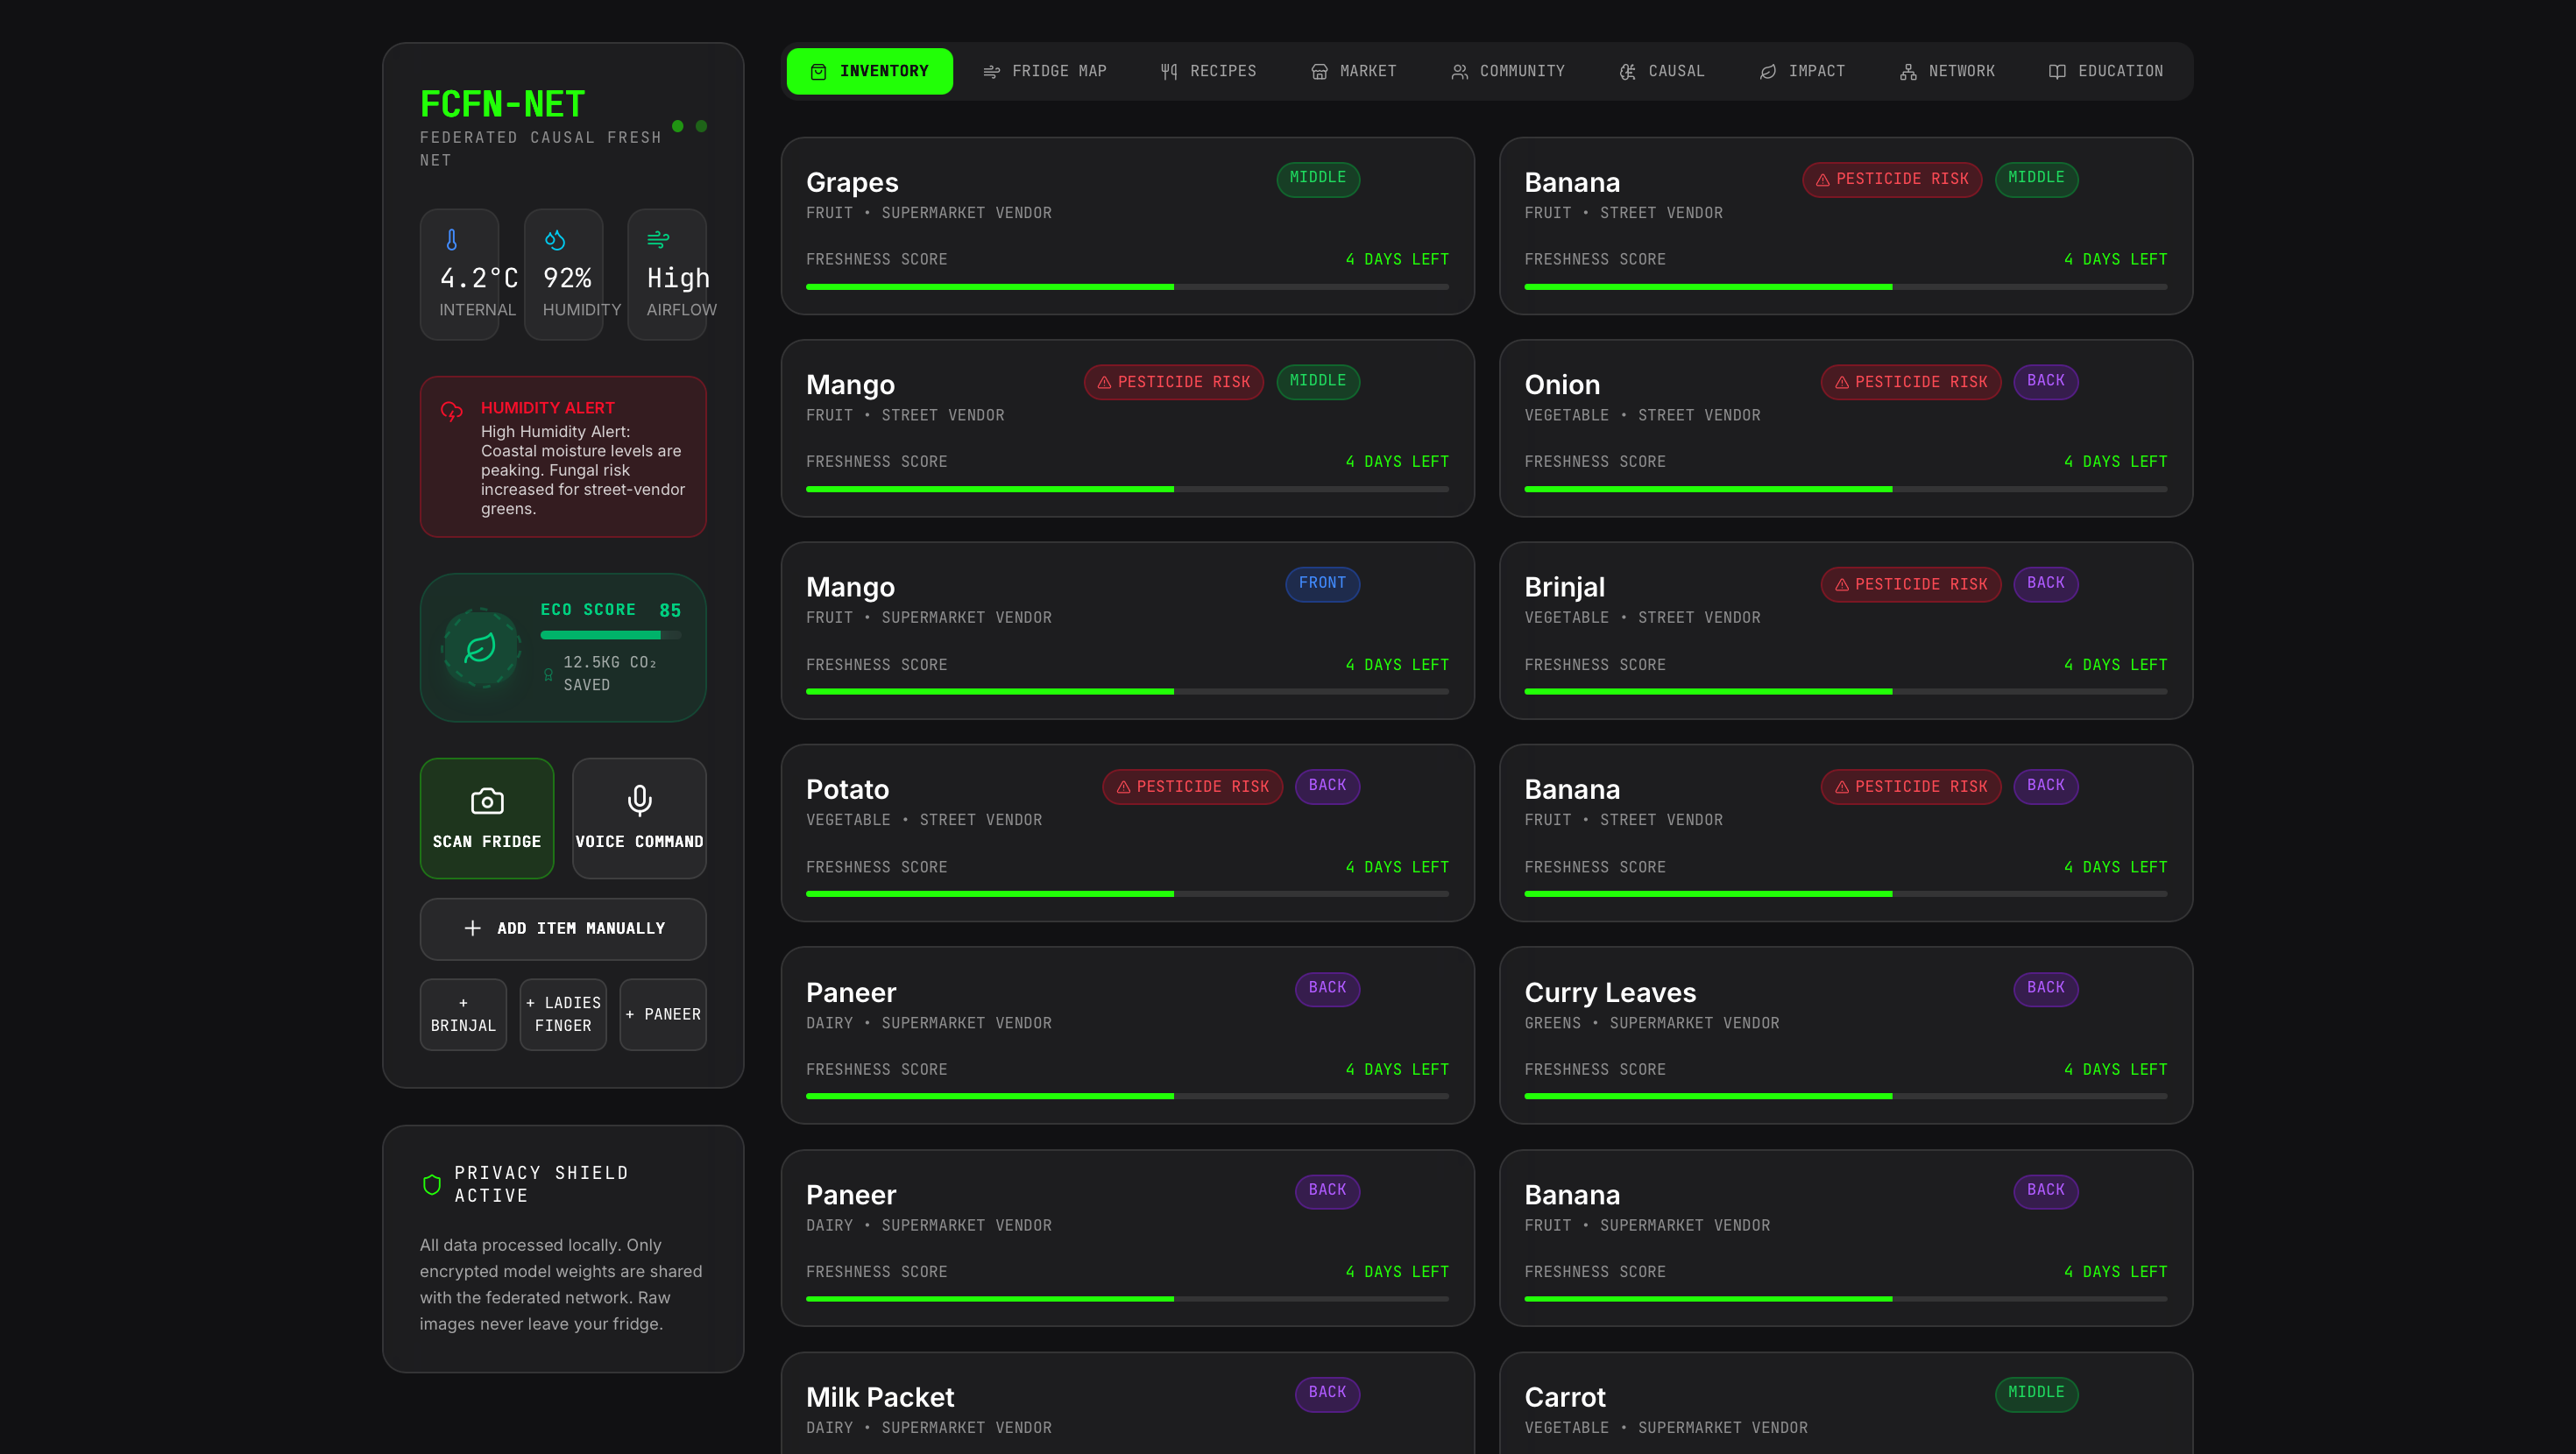
\includegraphics[width=0.85\textwidth]{inventory_dashboard.png}}
\caption{Module 1: Unified Inventory Intelligence Dashboard.}
\label{fig:module1}
\end{figure}

\subsection{Module 2: Fridge Spatial Mapping and Heatmap}
A custom SVG React component renders a 2D schematic of the fridge interior, divided into five thermal zones (door shelf, front shelf, middle shelf, back shelf, crisper drawer). Detected items are positioned within their detected zone as labeled icons. Each zone is overlaid with a color gradient representing the DHT22-derived temperature + humidity reading, augmented by calibrated zone offsets: door = +3.5°C, front = +2.1°C, middle = +0.5°C, back = setpoint, crisper = $-$0.8°C. Items positioned in thermally sub-optimal zones display a pulsing amber/red highlight animation. Hovering any item opens a tooltip showing its freshness score and the DoWhy ATE estimate for the recommended zone move. The heatmap provides an immediate, glanceable spatial summary that complements the data-heavy Module 1 table.

\begin{figure}[H]
\centering
\fbox{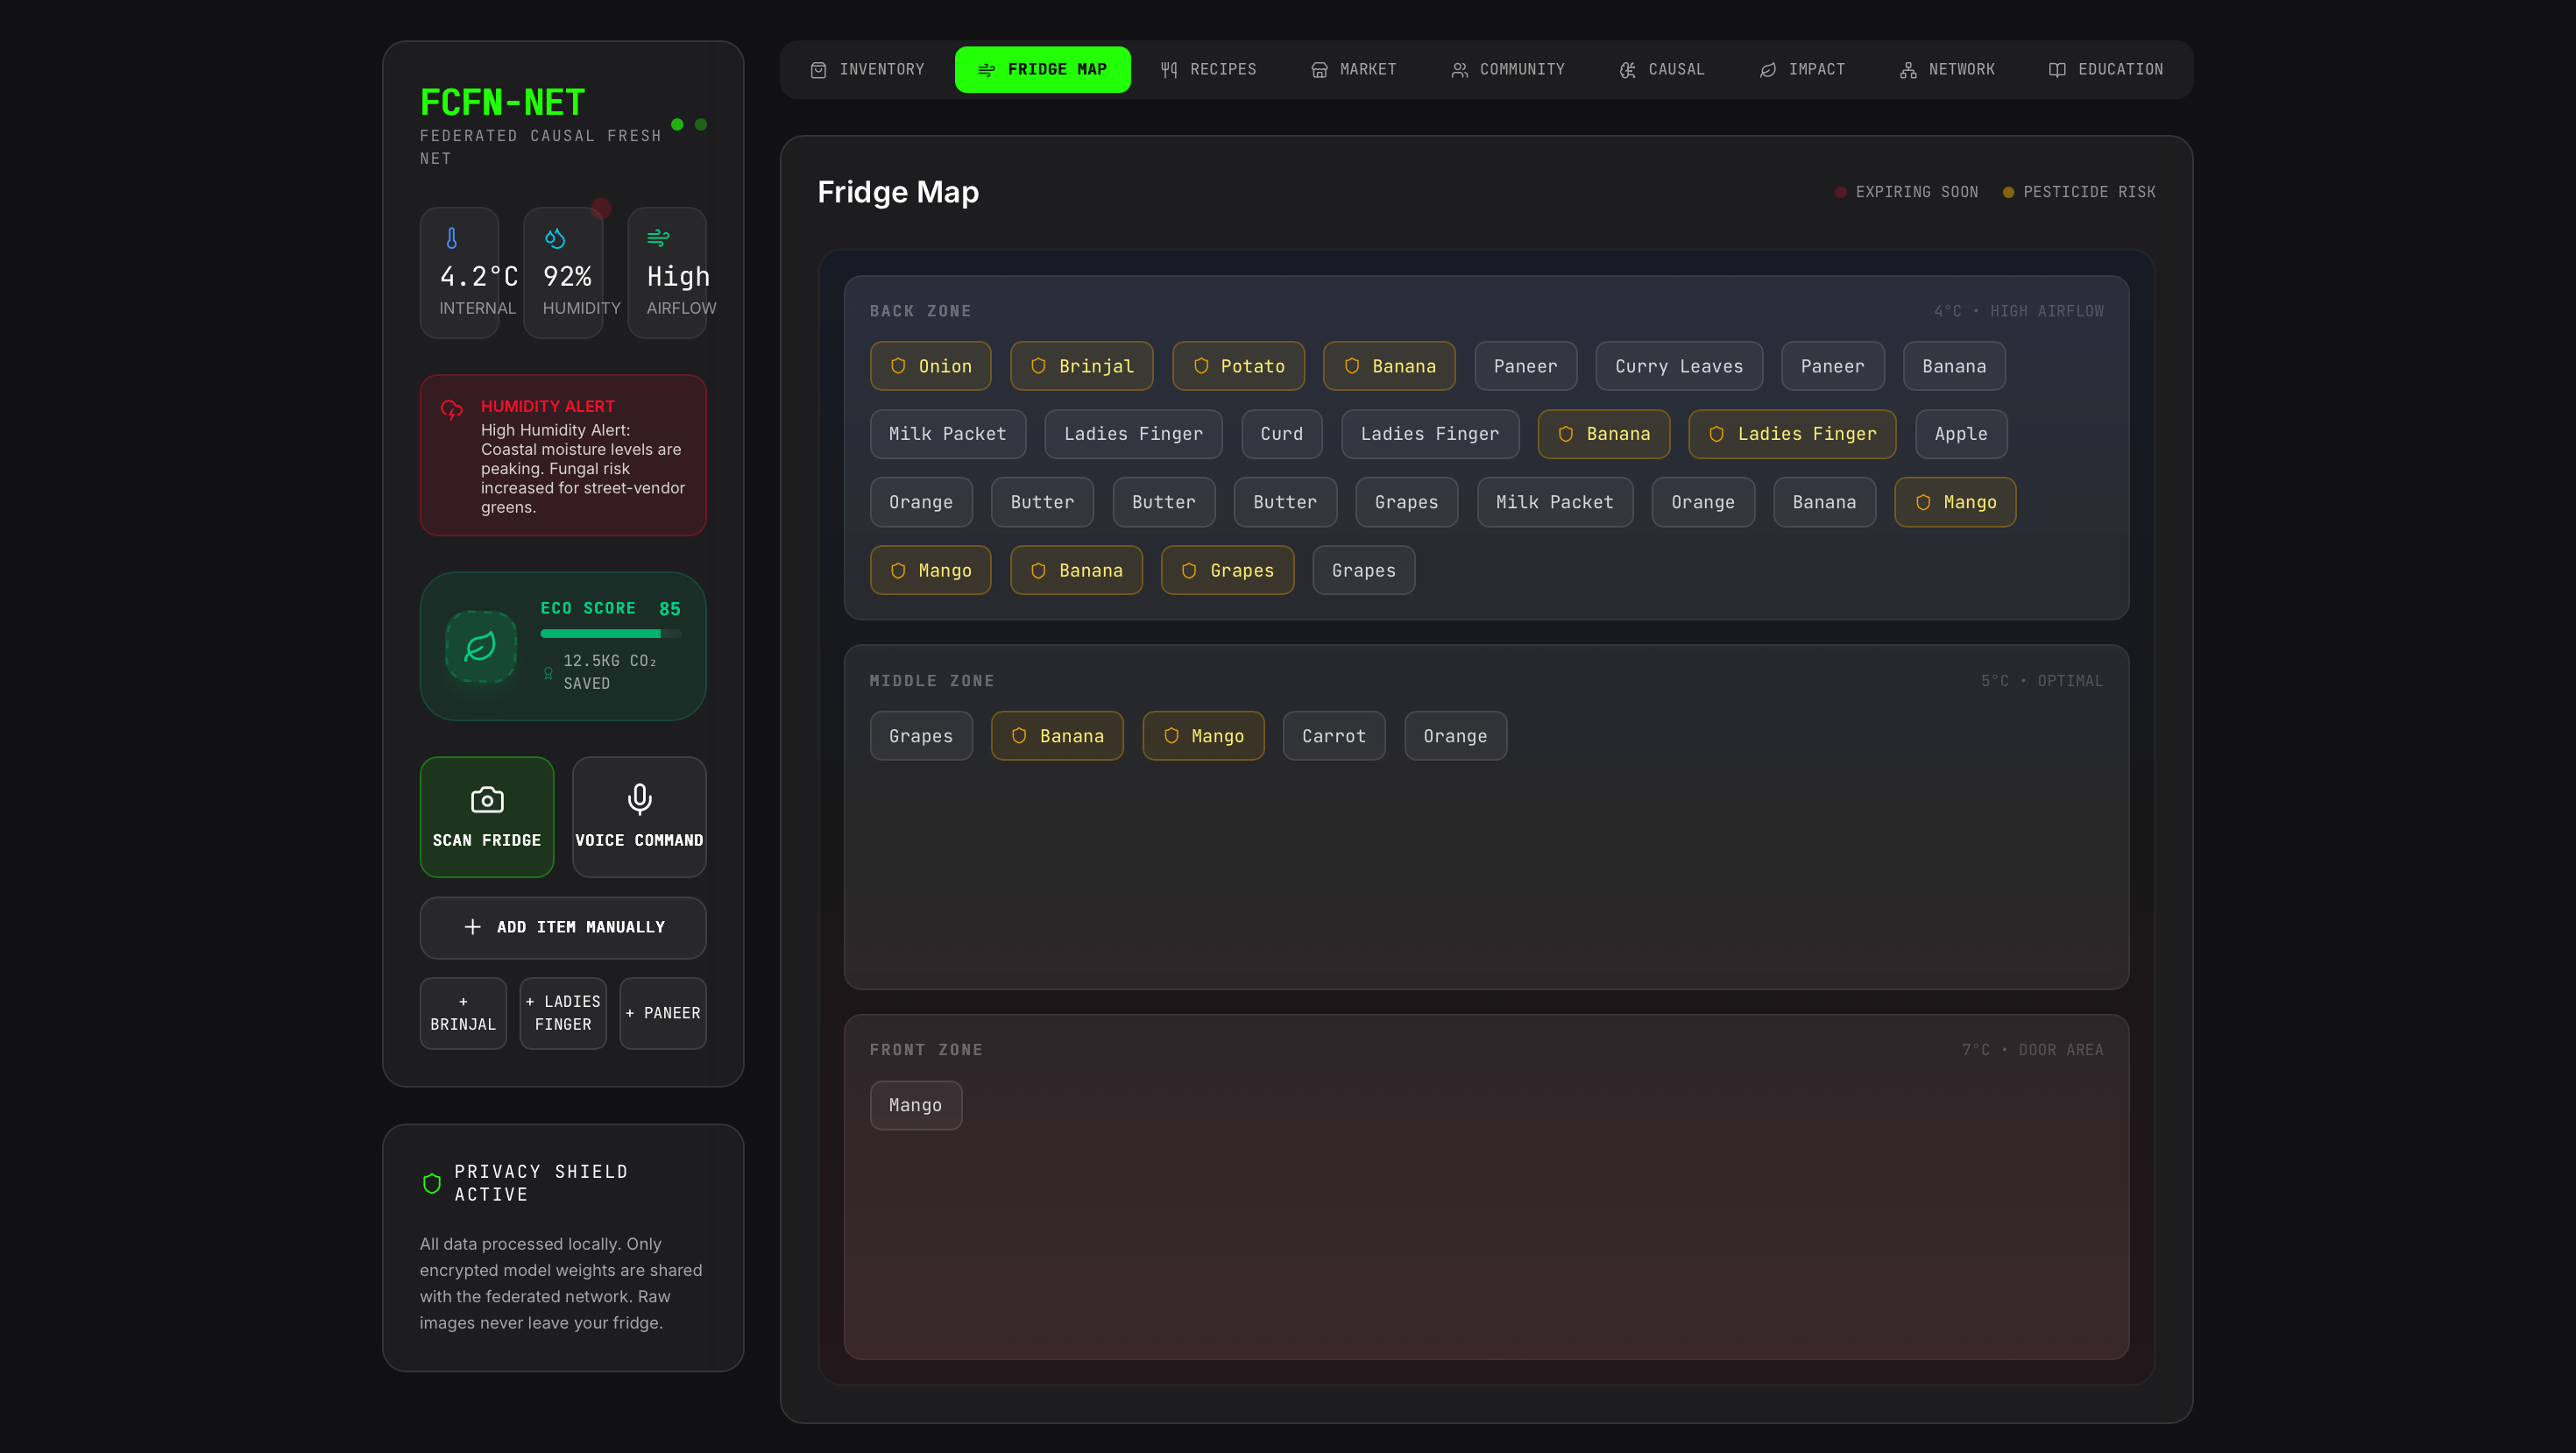
\includegraphics[width=0.85\textwidth]{fridge_map.png}}
\caption{Module 2: Fridge Spatial Heatmap and Thermal Zone Visualization.}
\label{fig:module2}
\end{figure}

\subsection{Module 3: AI-Driven Waste Reduction (Gemini Pro)}
A FastAPI \texttt{BackgroundTask} polls \texttt{inventory\_items} every 4 hours for items whose freshness score has fallen below 40\%. All qualifying items are batched into a single Gemini Pro 1.5 API call. The prompt specifies: ingredient list with freshness percentages; mandatory inclusion of all near-expiry items; Tamil Nadu cuisine style preference (Kuzhambu, Kootu, Rasam, Poriyal, Pongal, Sambar, Porridge); a food safety tip per ingredient; and a cook-time estimate. The Gemini response is stored in \texttt{recipe\_logs} and rendered in a recipe card UI with the Gemini branding badge and a ``Use-By Alert'' countdown timer.

\begin{figure}[H]
\centering
\fbox{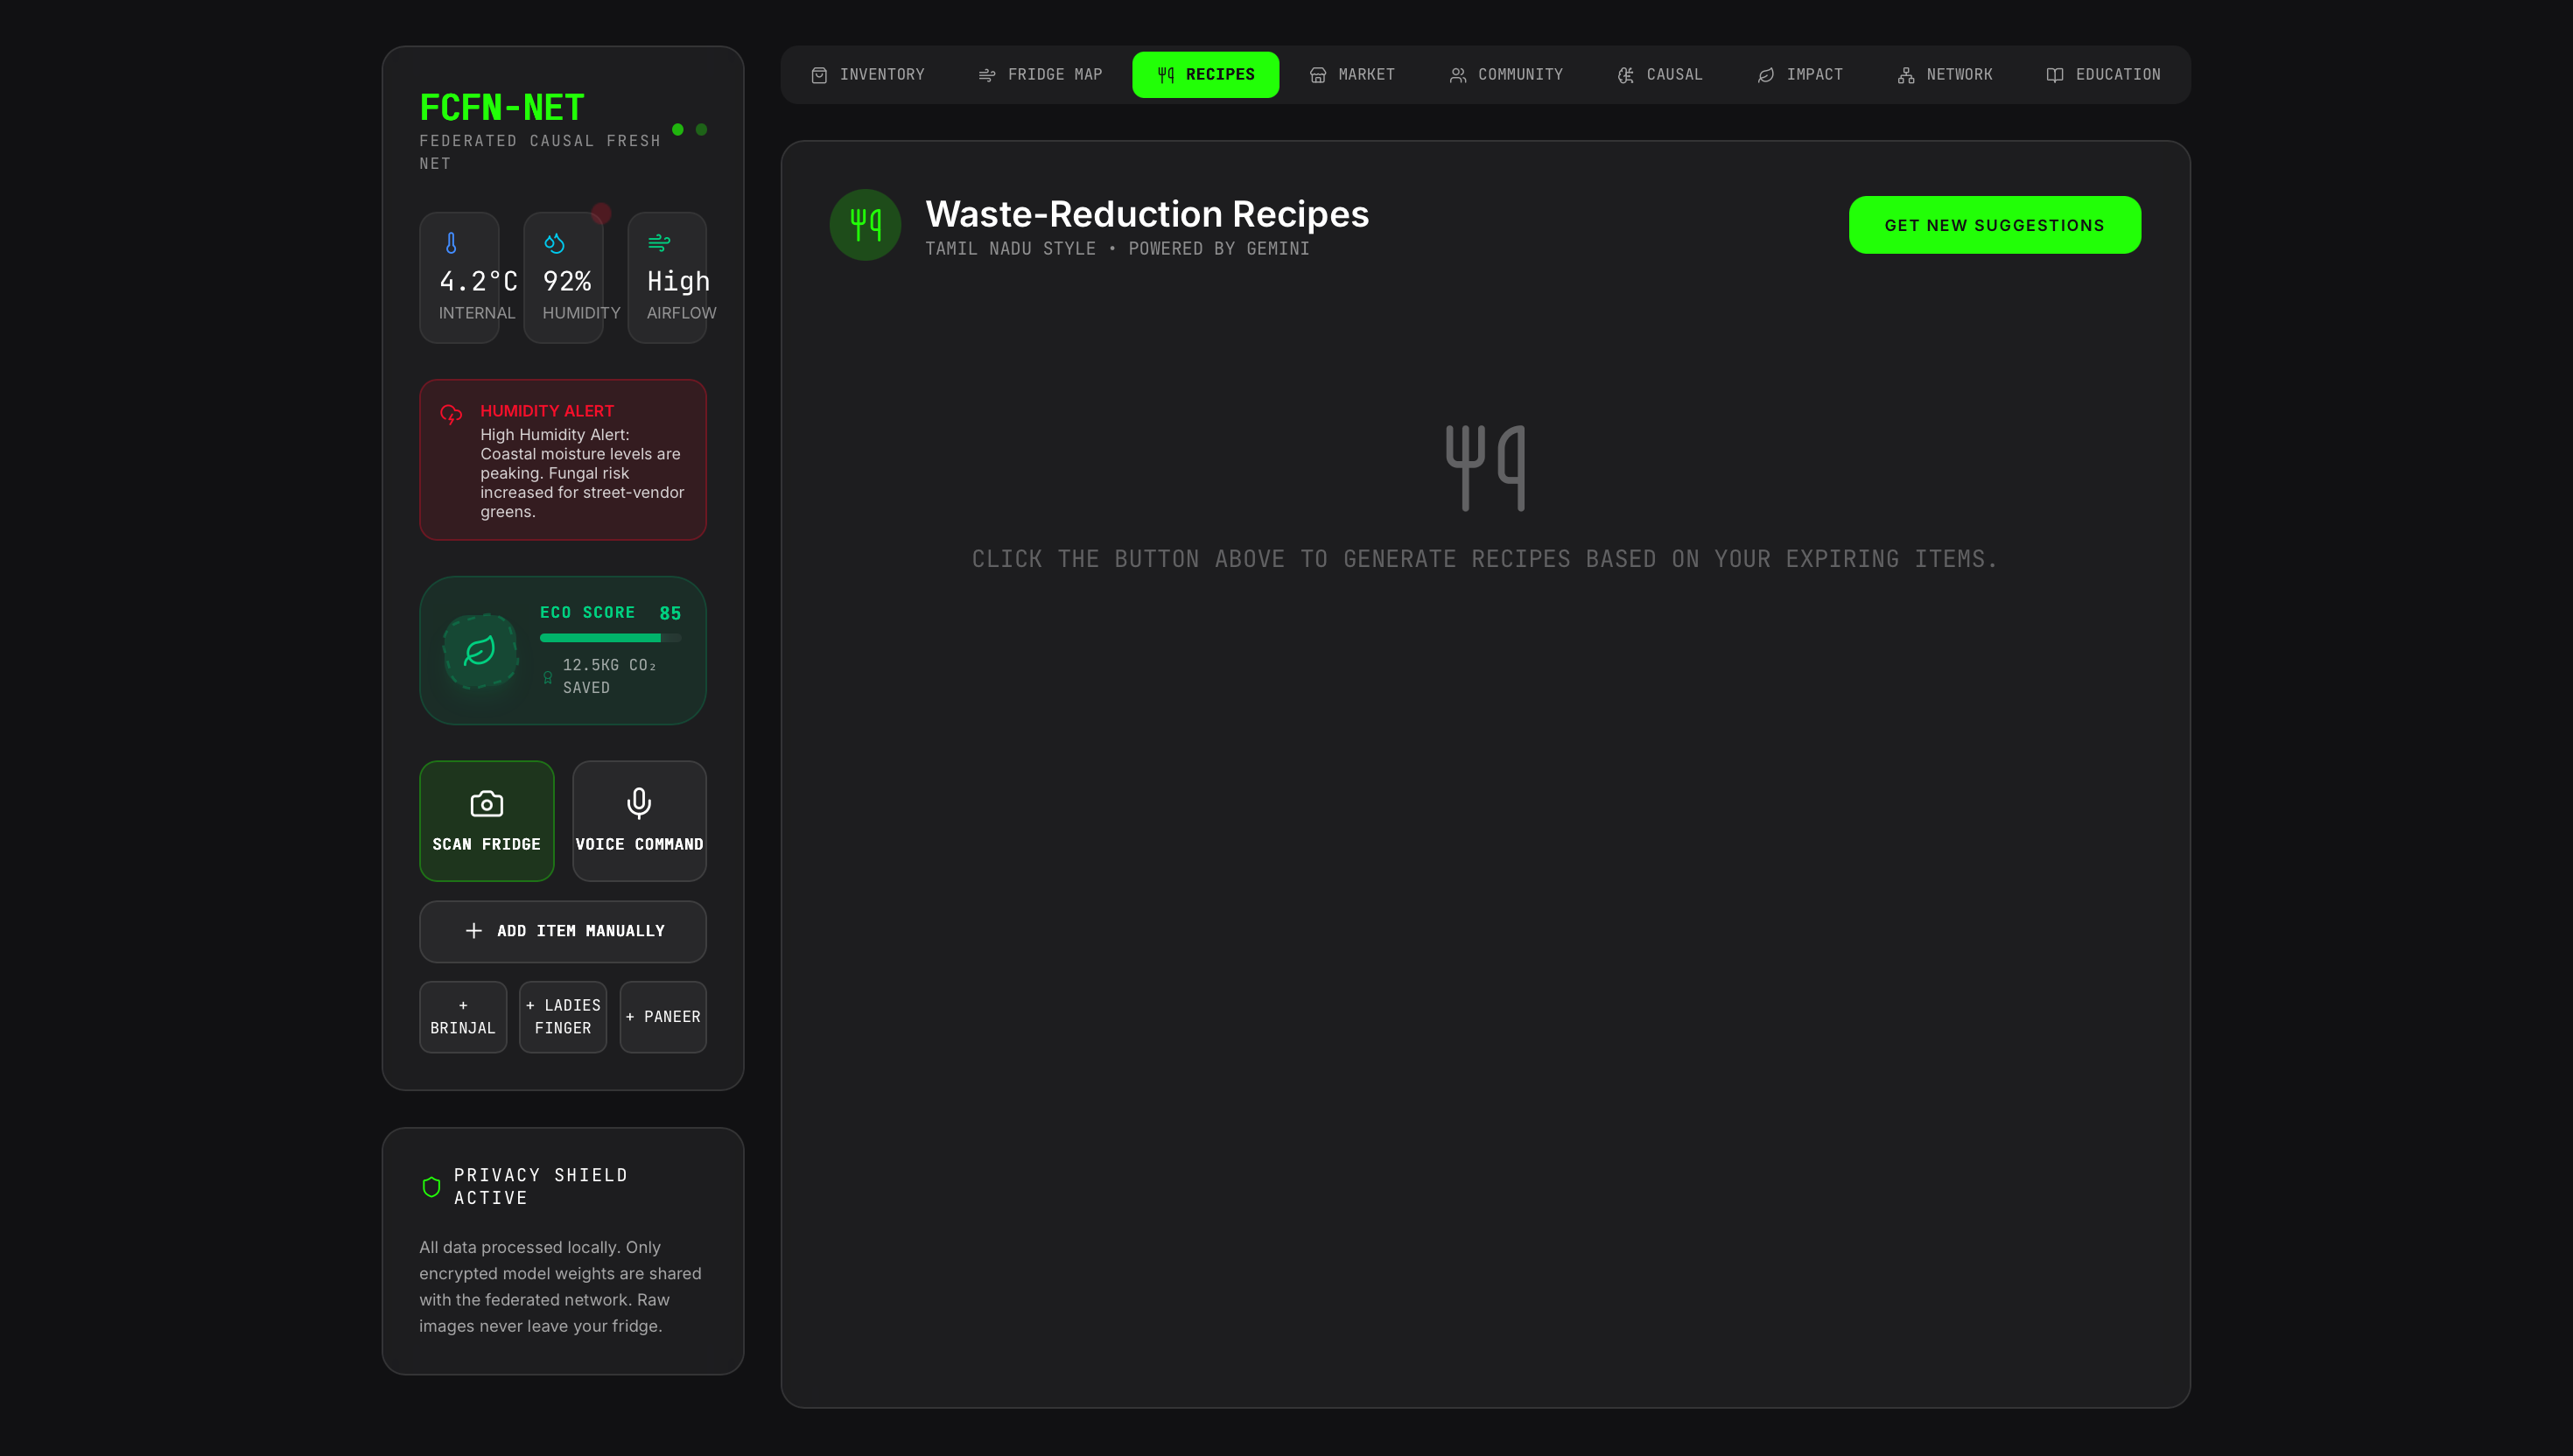
\includegraphics[width=0.85\textwidth]{recipes_ai.png}}
\caption{Module 3: AI-Driven Zero-Waste Recipe Generation.}
\label{fig:module3}
\end{figure}

\subsection{Module 4: Consumption Forecasting and Market Intelligence}
Sequential scan data is used to estimate per-item consumption rates via linear regression on quantity-over-time. The model projects a ``zero-stock deadline'' for each item. This is compared against the freshness-decay-projected expiry (Equation~\ref{eq:decay}); the earlier of the two becomes the displayed ``action deadline.'' A secondary panel displays a community-contributed price index for 20+ Tamil Nadu produce items sourced weekly from Koyambedu market rate data, providing shopping cost context alongside consumption forecasts.

\begin{figure}[H]
\centering
\fbox{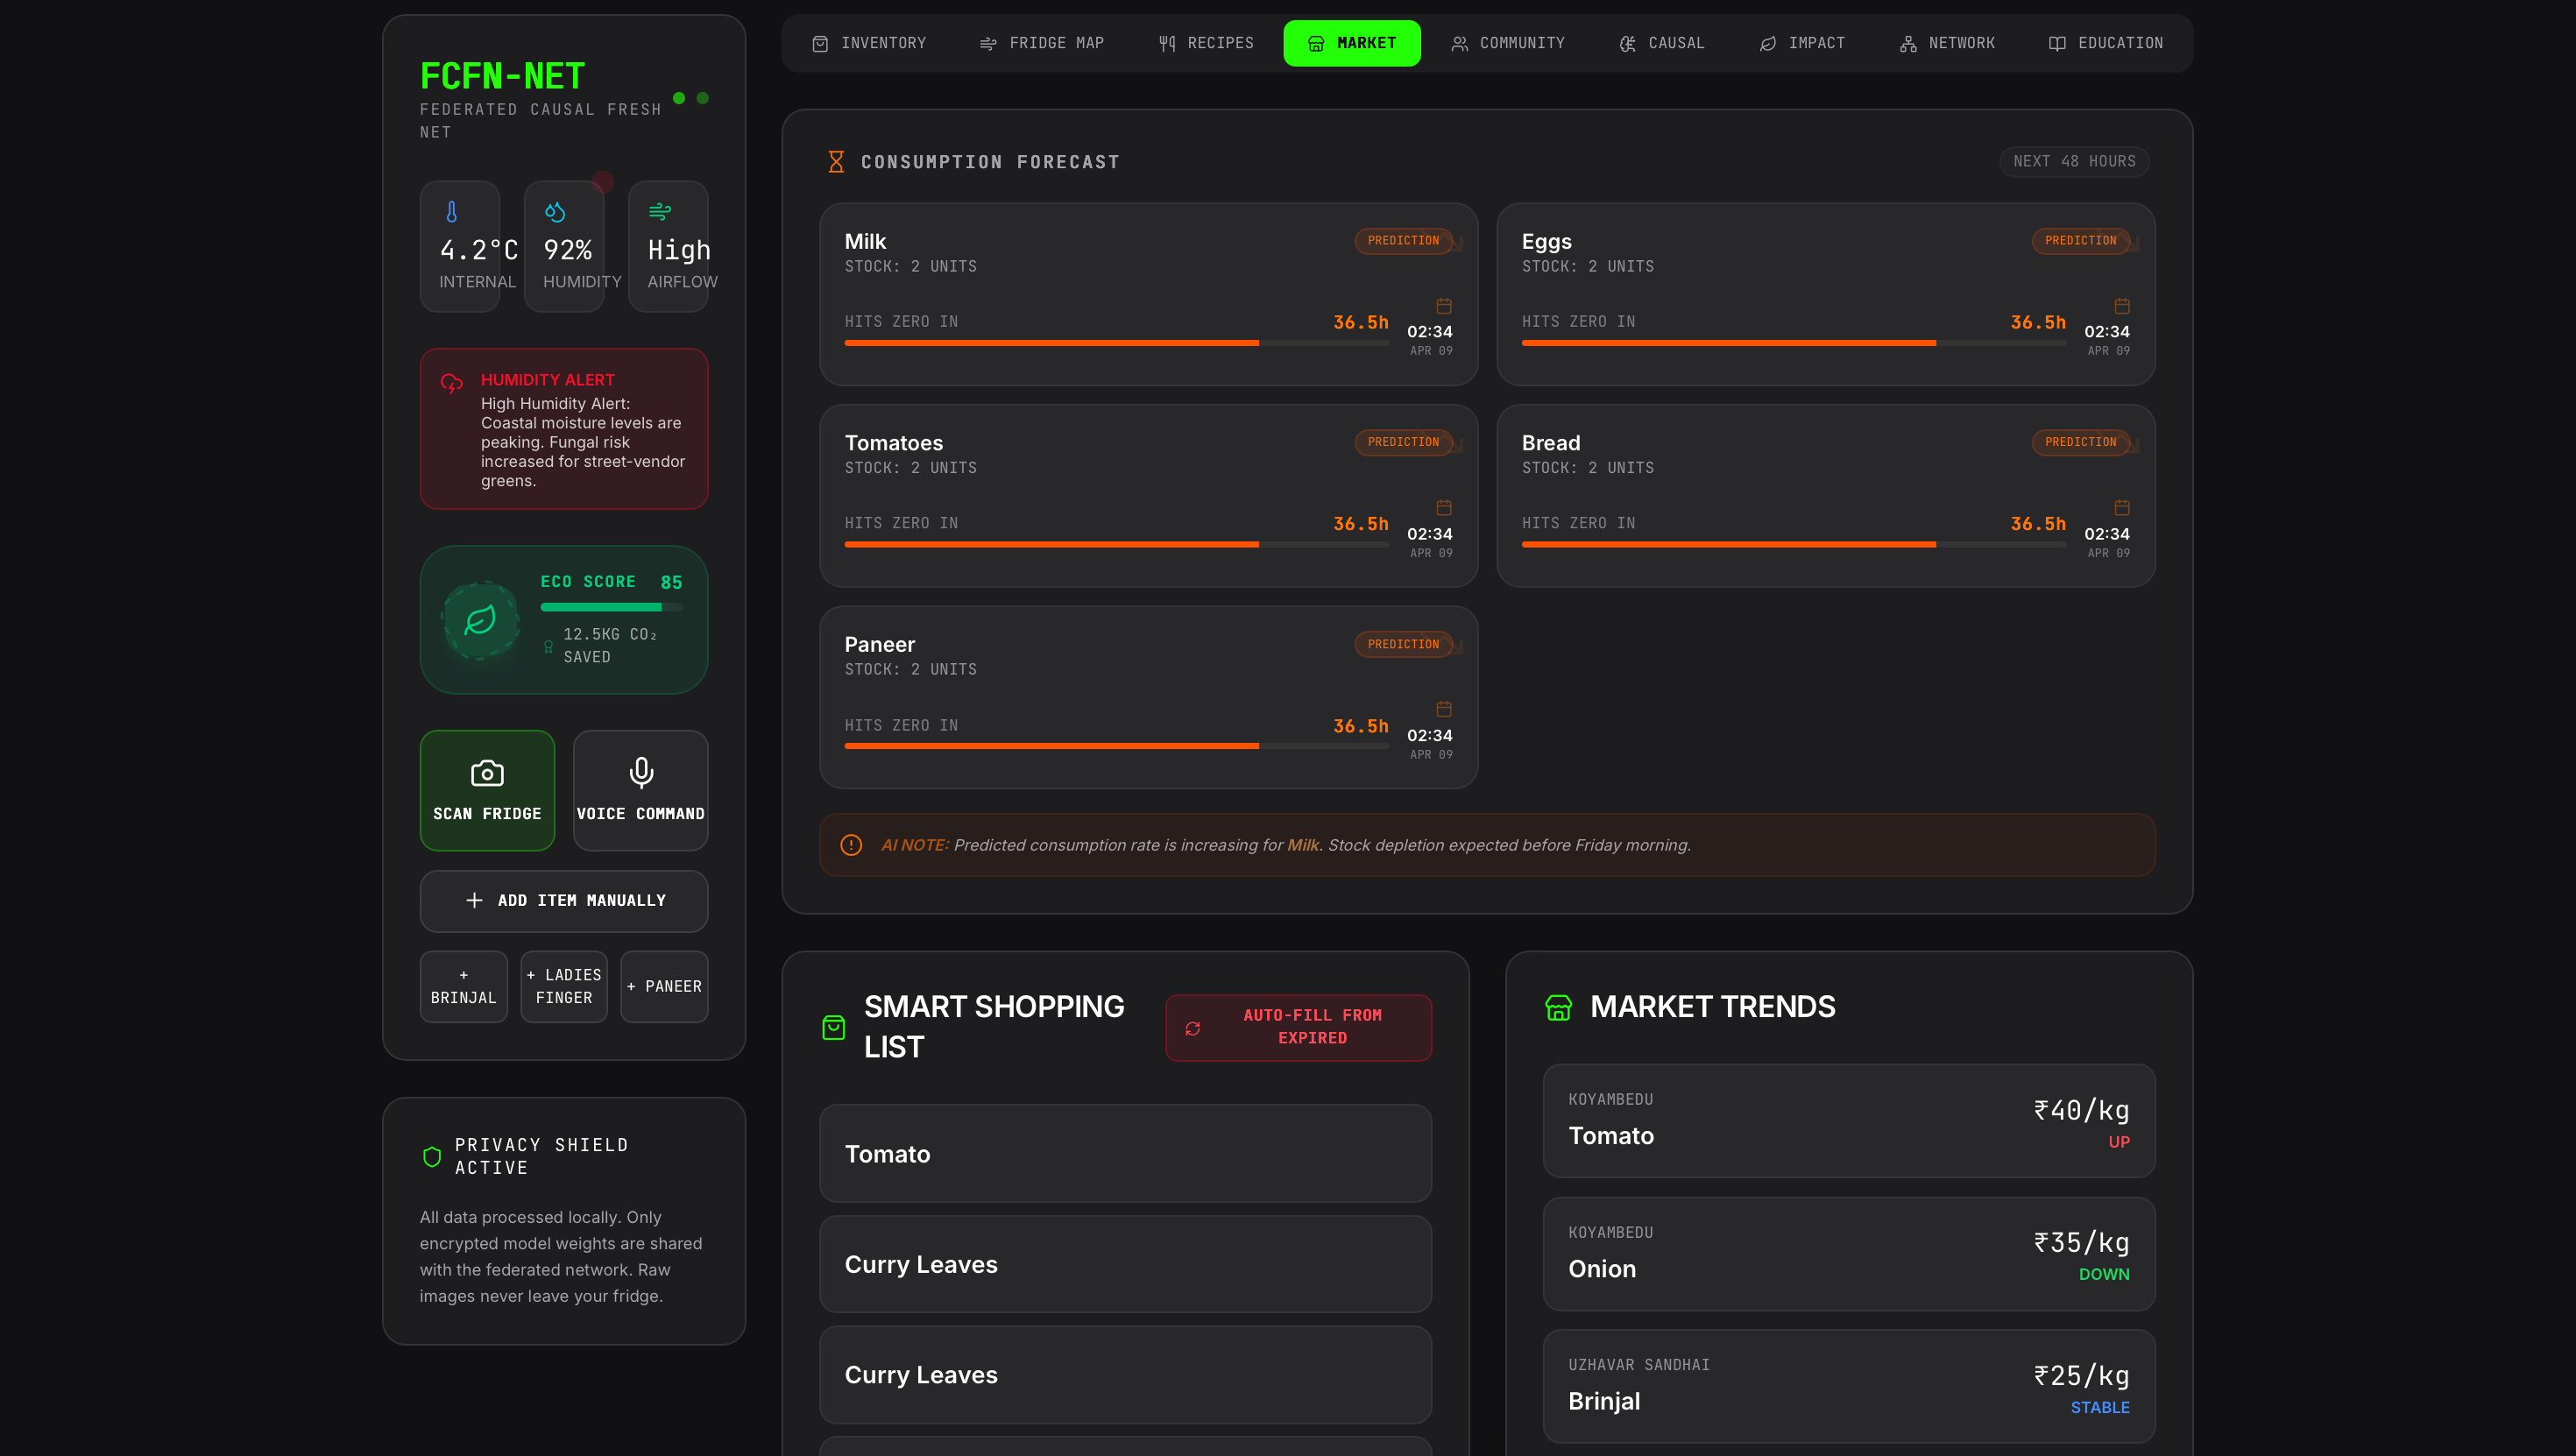
\includegraphics[width=0.85\textwidth]{market_forecast.png}}
\caption{Module 4: Consumption Forecasting and Market Price Analytics.}
\label{fig:module4}
\end{figure}

\subsection{Module 5: Community Hub — Privacy-First Food Exchange}
The Community Hub implements a decentralized, privacy-preserving P2P surplus food exchange board. All listings transmit zero Personally Identifiable Information: items are listed only by food category, approximate quantity descriptor (``small bunch'', ``2 packets''), and a hashed 2km-radius neighborhood zone identifier — never an address, name, or phone number. Claiming a listing initiates a one-time handshake entirely within the local network. The module also surfaces anonymized aggregated freshness trends from all participating nodes (e.g., ``63\% of coriander in Zone 7 is below 50\% freshness — quality likely dropping at source market''), providing actionable market-level intelligence. All community data exchange complies architecturally with India's DPDPA 2023.

\begin{figure}[H]
\centering
\fbox{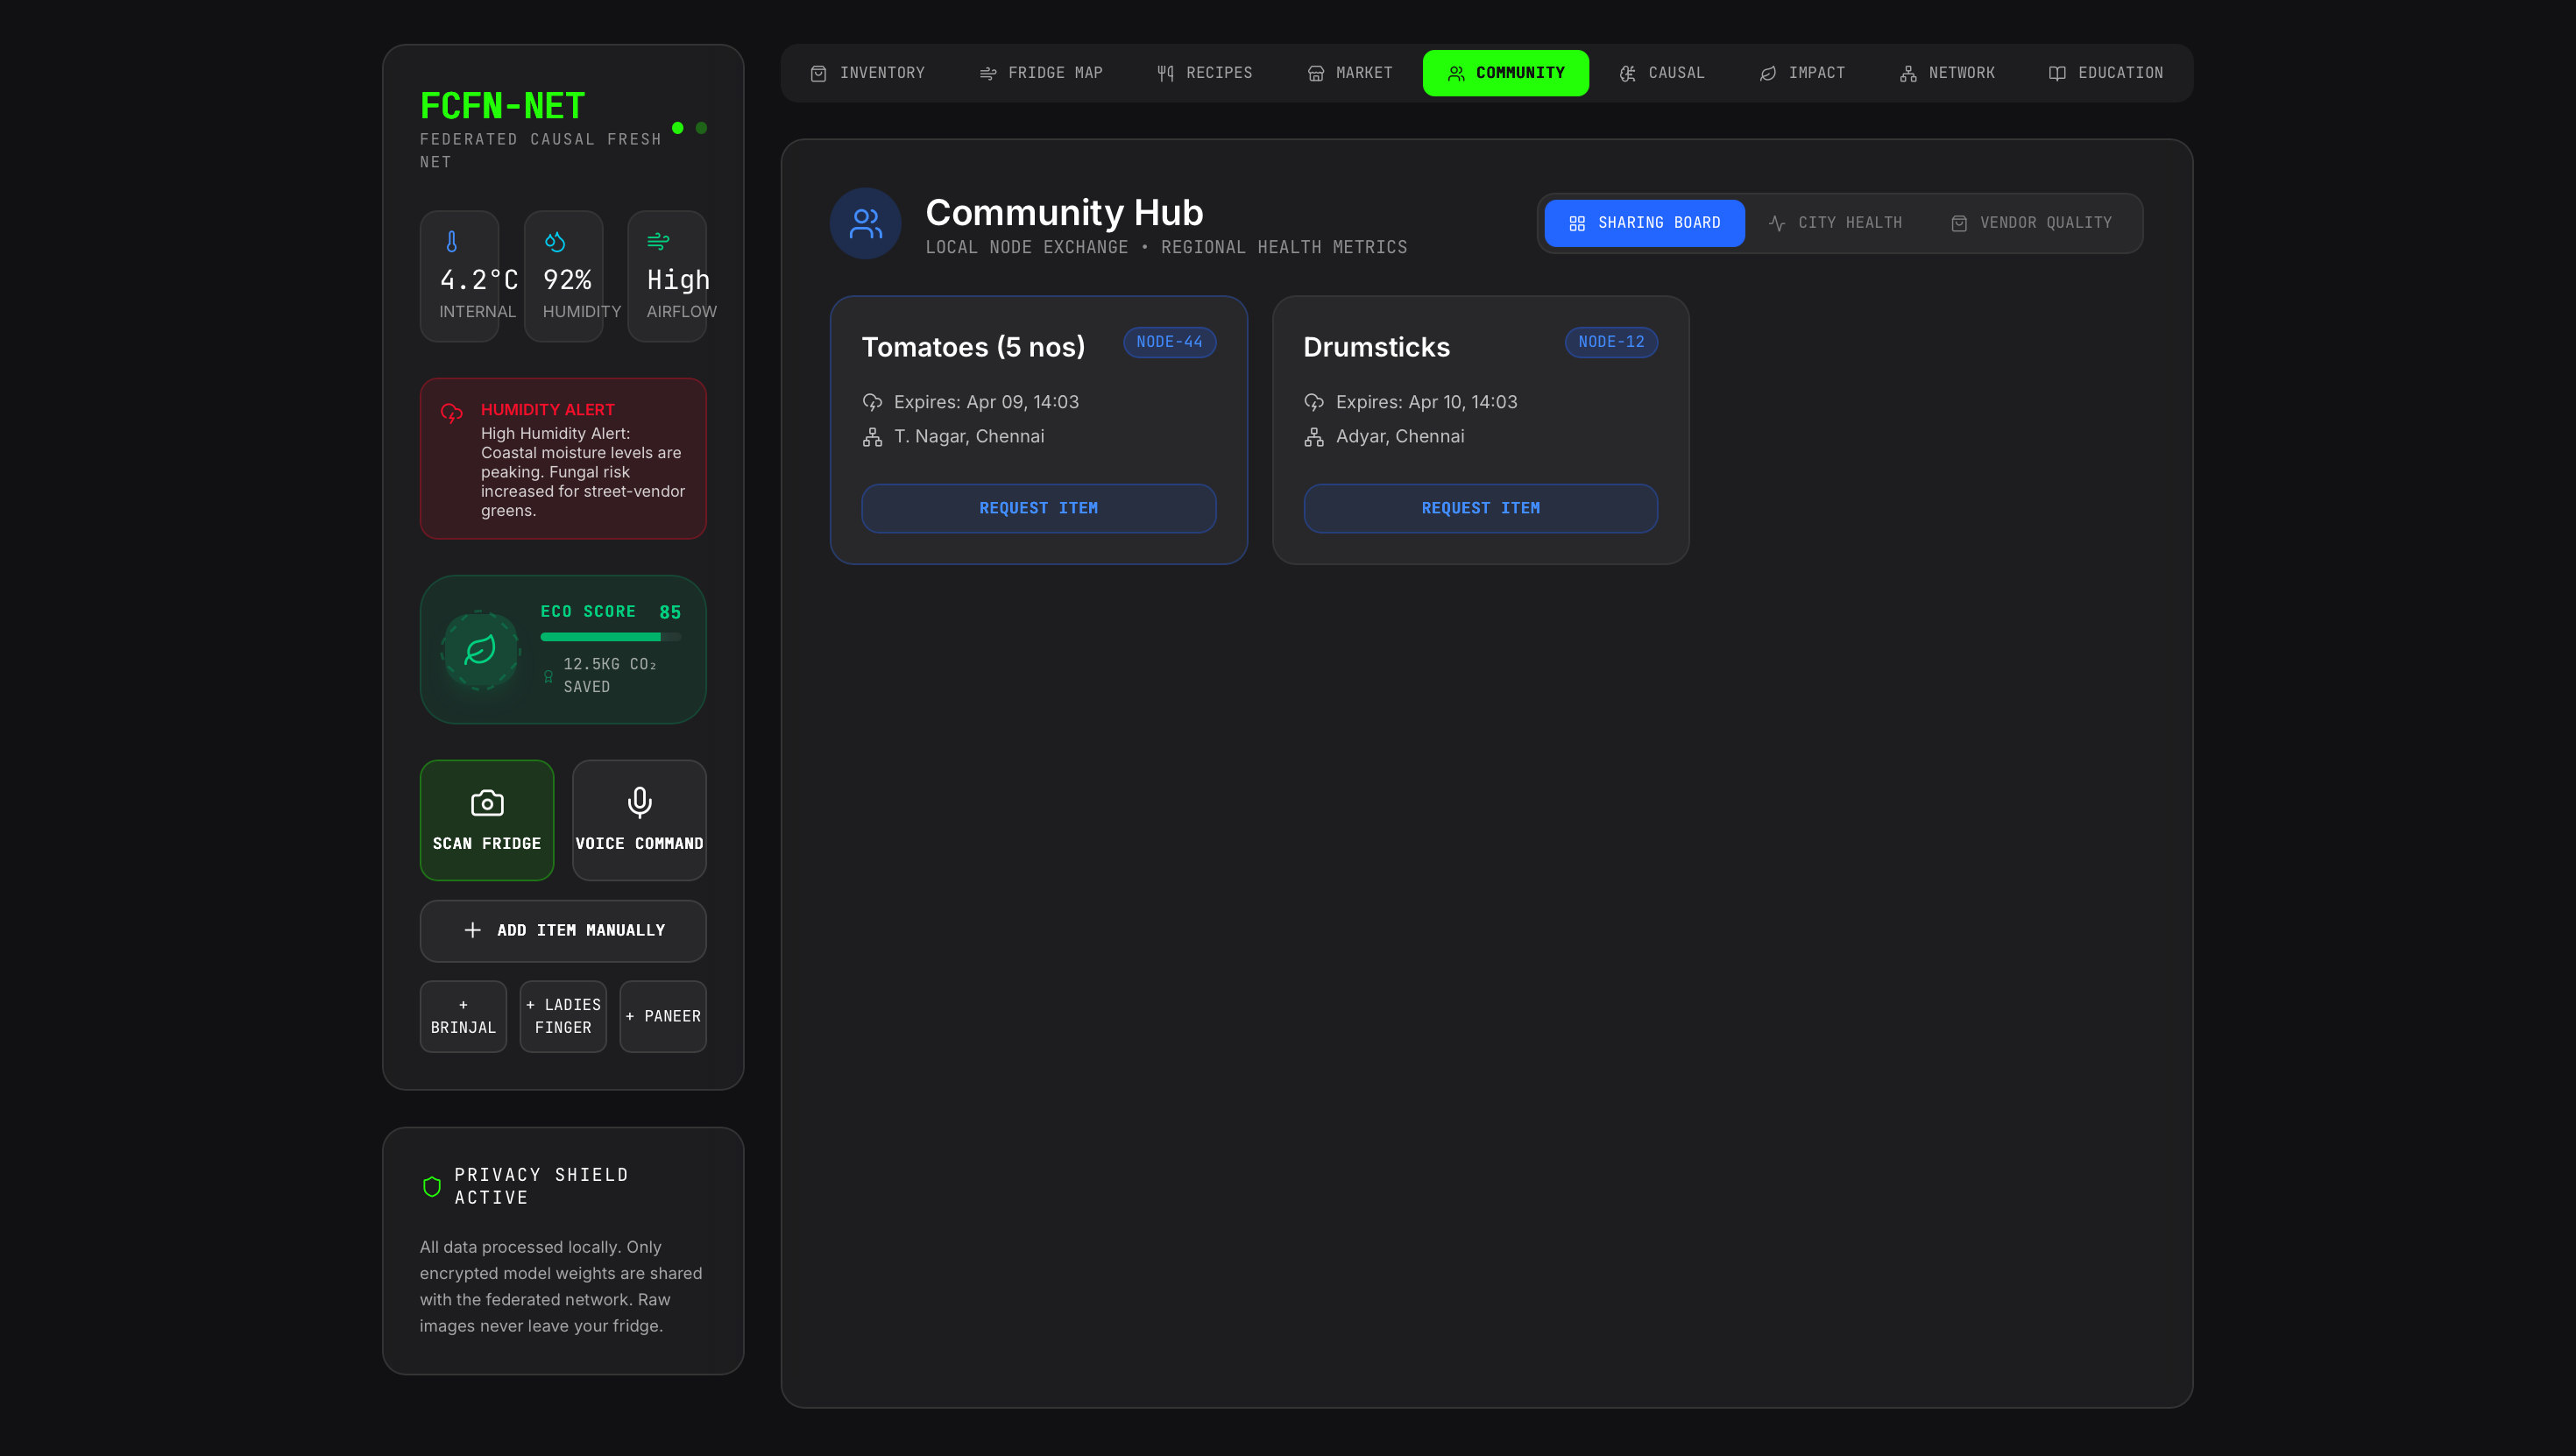
\includegraphics[width=0.85\textwidth]{community_hub.png}}
\caption{Module 5: Privacy-First P2P Community Food Exchange.}
\label{fig:module5}
\end{figure}

\subsection{Module 6: Causal Spoilage Simulator}
An interactive ``what-if'' counterfactual interface. The user selects any tracked inventory item from a dropdown and a target zone from a visual zone selector. On submission, a POST request to \texttt{/api/causal} executes the full DoWhy pipeline (Listing~3.4) using the past 6 months of node-local historical scan data as the observational dataset. The result — e.g., ``Moving Tomato from Front Shelf to Back Shelf: +4.55 days [95\% CI: 3.87, 5.23] — Refutation: PASSED'' — is displayed alongside a dual Recharts \texttt{AreaChart} overlaying the current-zone freshness decay curve against the projected post-intervention decay curve per Equation~\ref{eq:decay}.

\begin{figure}[H]
\centering
\fbox{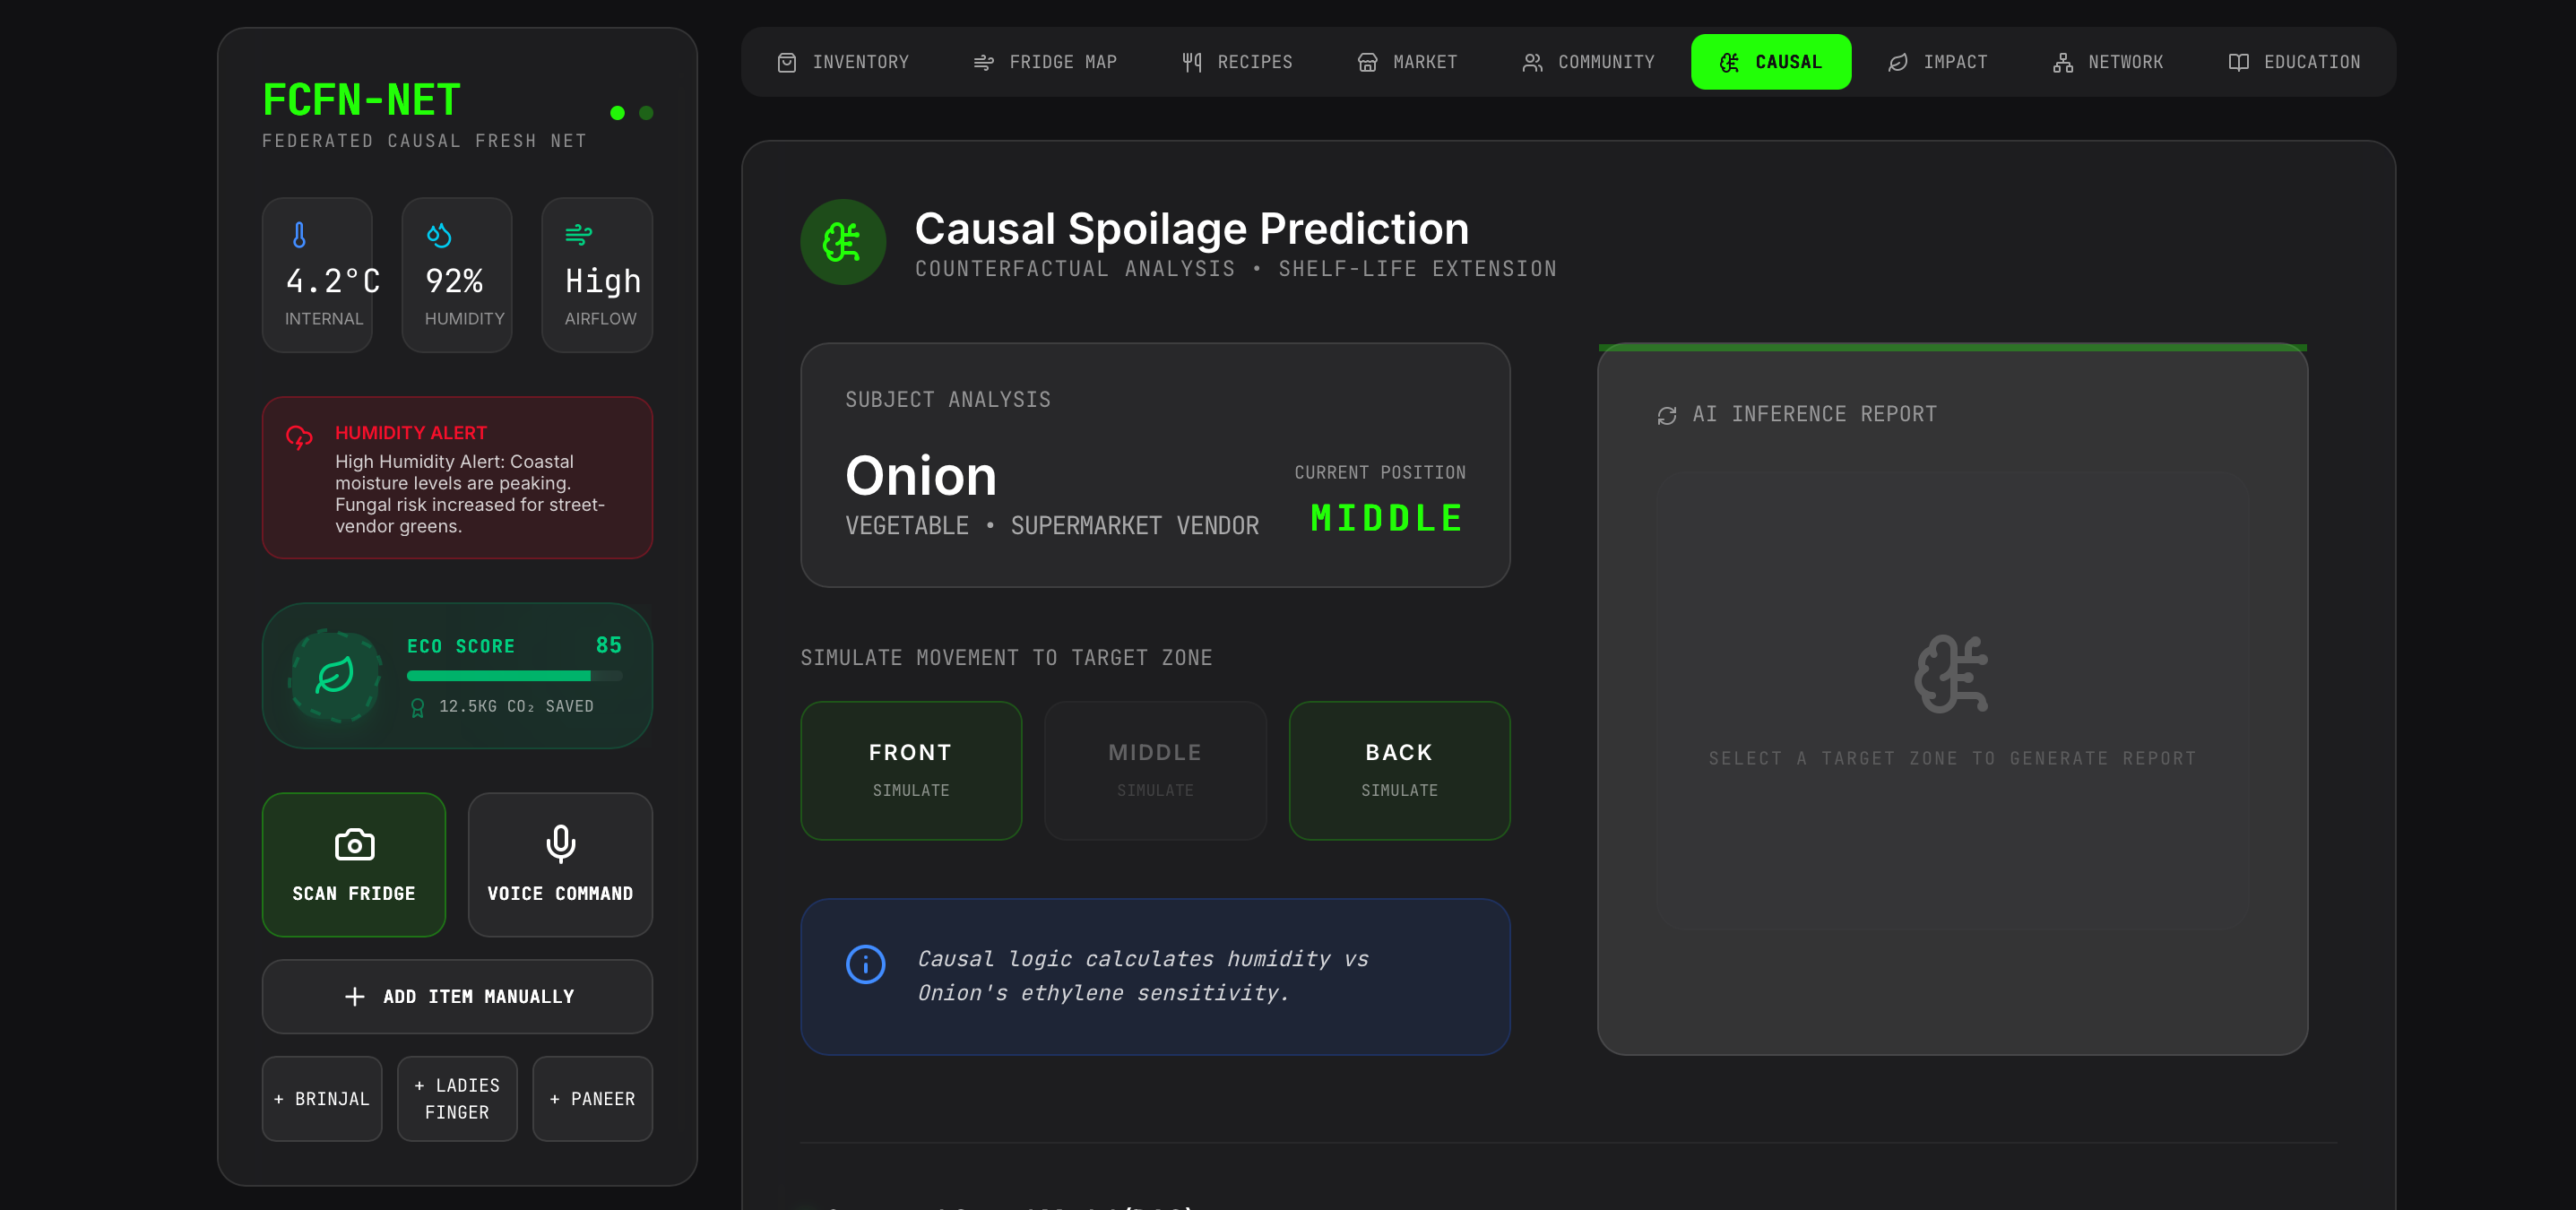
\includegraphics[width=0.85\textwidth]{causal_spoilage.png}}
\caption{Module 6: Counterfactual Causal Spoilage Simulator.}
\label{fig:module6}
\end{figure}

\subsection{Module 7: Sustainability Impact Tracker}
Converts food-rescue actions into quantified environmental metrics using IPCC AR6 lifecycle emission factors (EFs). The CO\textsubscript{2} equivalent prevented by rescuing a batch of items is computed as:
\begin{equation}
    CO_2^{prevented} = \sum_{i \in \text{rescued}} m_i \cdot EF_i
\end{equation}
where $m_i$ is the rescued mass (kg) and $EF_i$ is the item-specific IPCC AR6 lifecycle emission factor (e.g., tomatoes: 1.44\,kgCO\textsubscript{2}e/kg; paneer: 11.4\,kgCO\textsubscript{2}e/kg; coriander: 3.2\,kgCO\textsubscript{2}e/kg). A gamified leaderboard ranks participating nodes by monthly CO\textsubscript{2} savings and food-kilograms rescued. The module also maintains an ``equivalent trees planted'' and ``equivalent car km avoided'' display to provide intuitive scale to the carbon metrics.

\begin{figure}[H]
\centering
\fbox{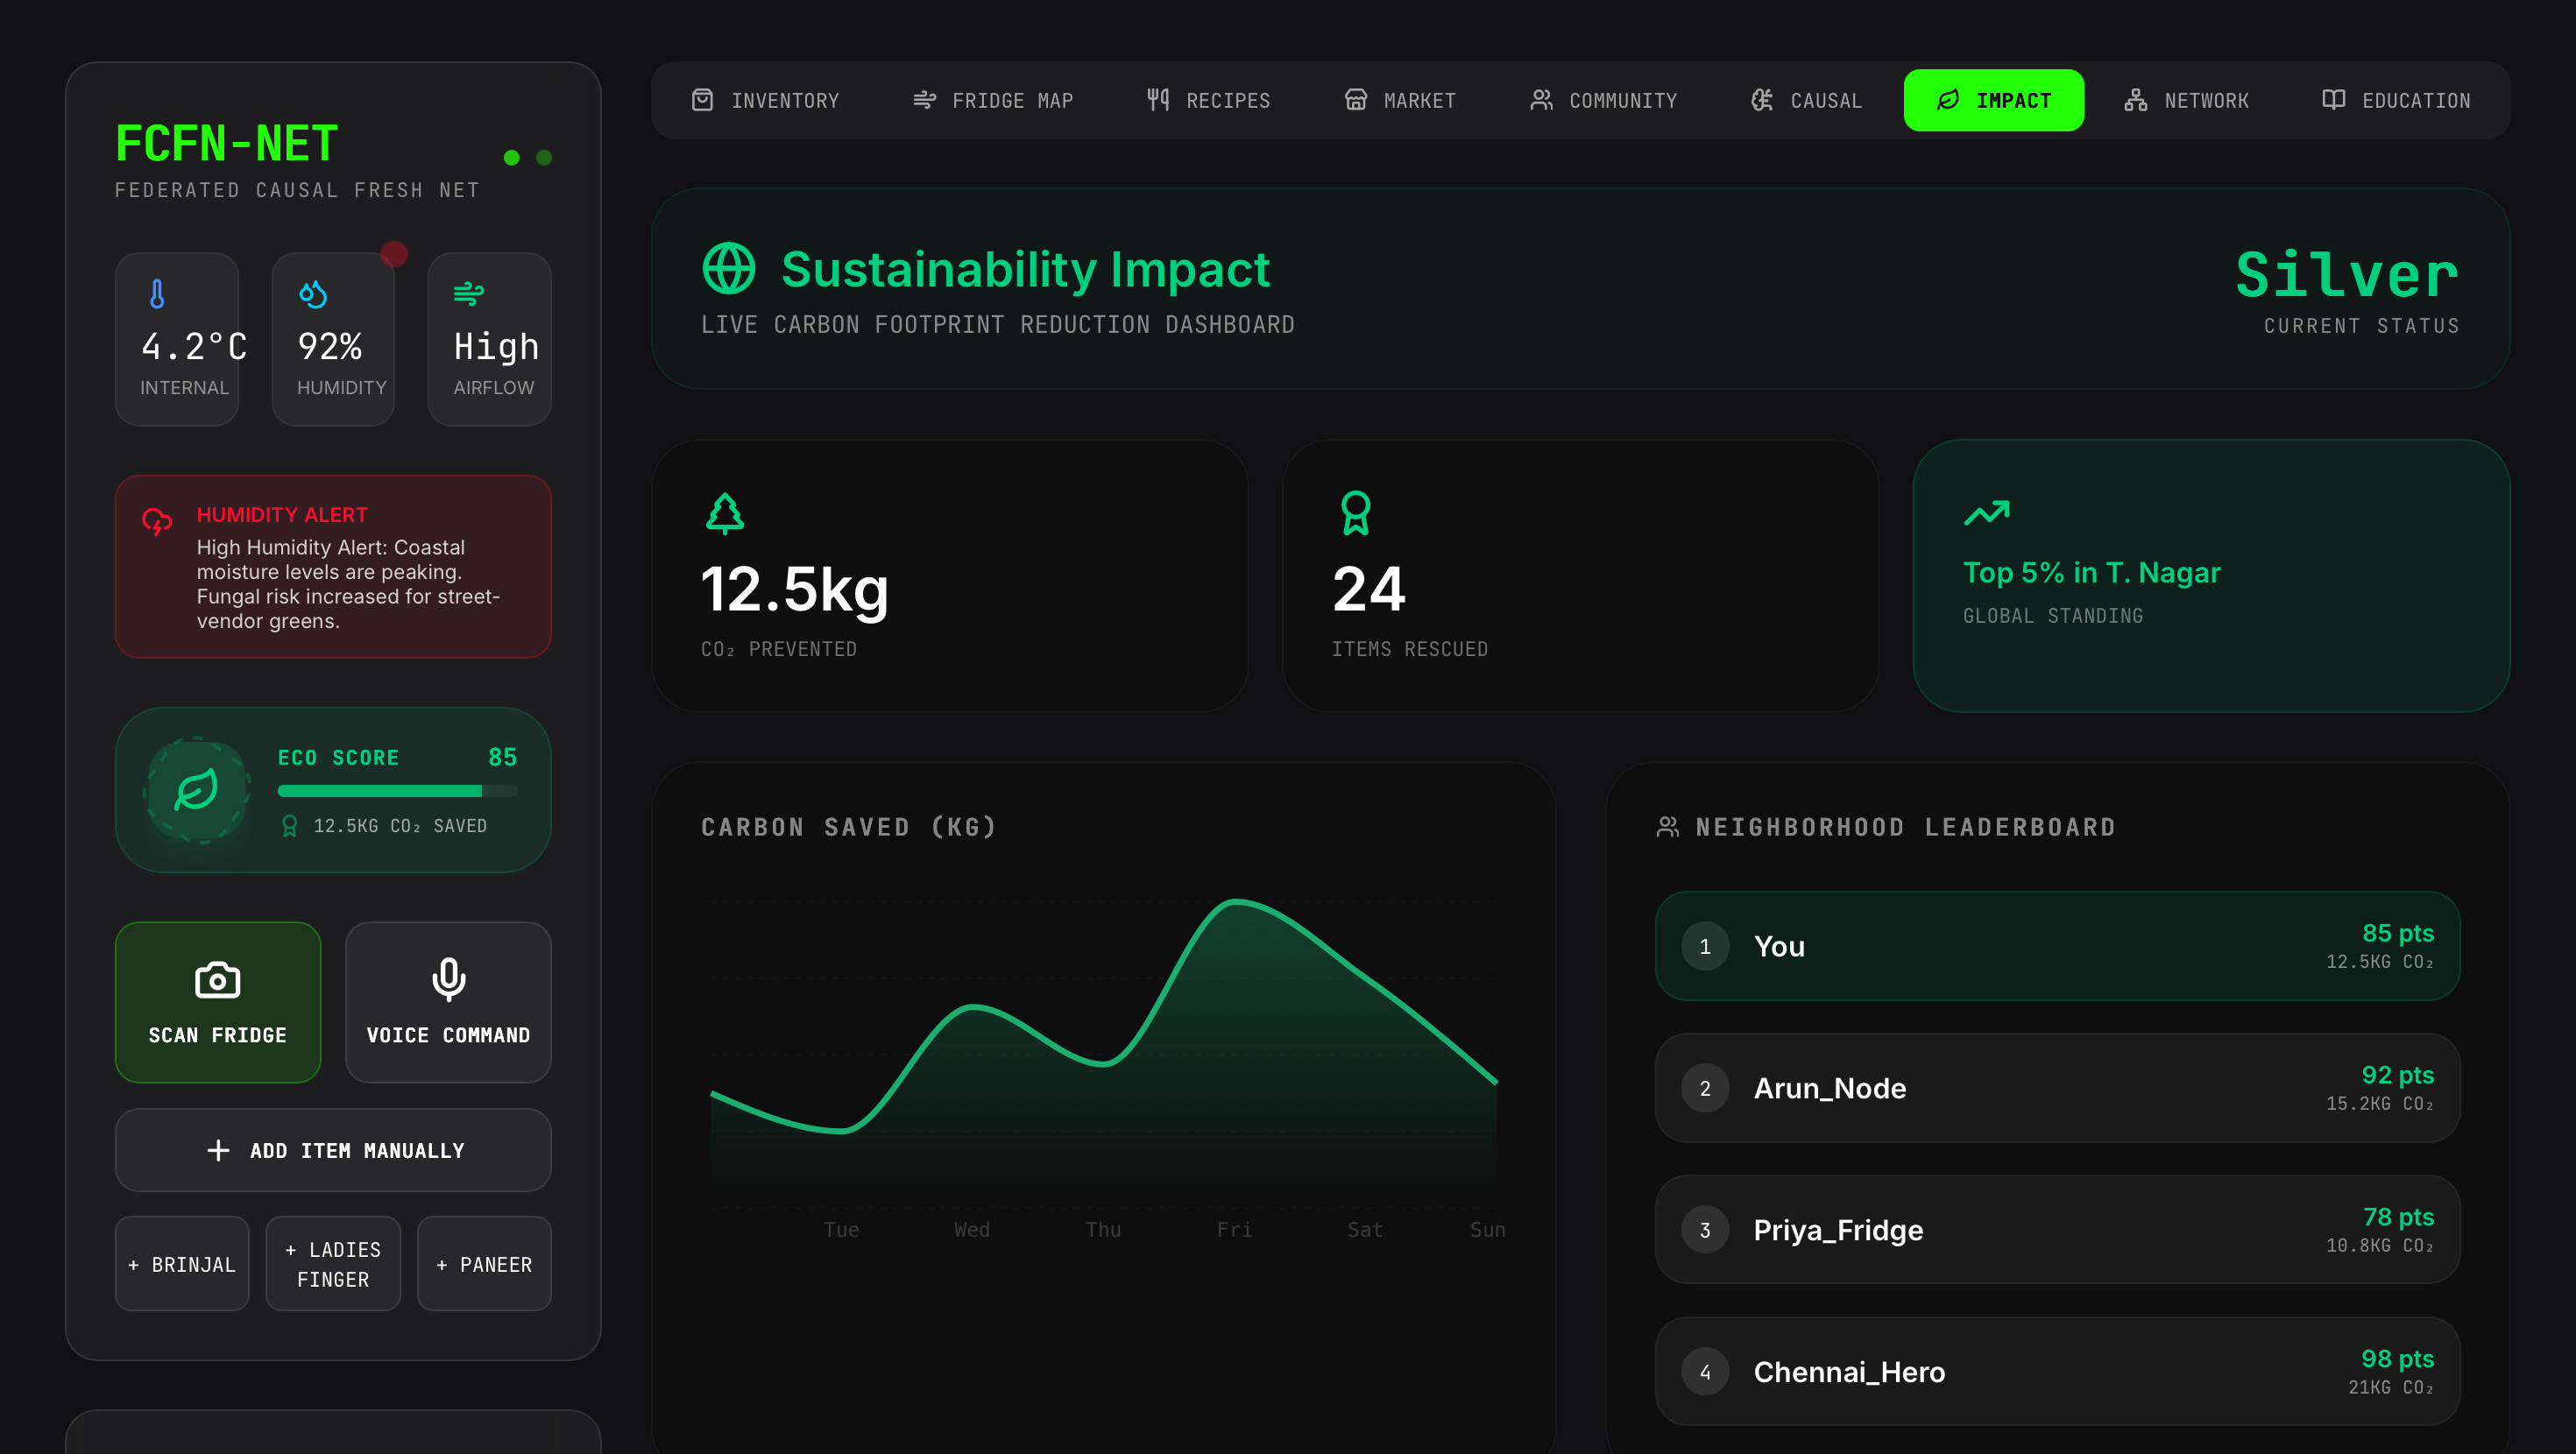
\includegraphics[width=0.85\textwidth]{sustainability_impact.png}}
\caption{Module 7: Carbon Offset and Food-Rescue Sustainability Tracker.}
\label{fig:module7}
\end{figure}

\subsection{Module 8: Federated Network Activity Dashboard}
Provides a real-time window into the otherwise invisible federated learning process, making the privacy guarantee tangible and verifiable for users. A Recharts \texttt{LineChart} plots global model accuracy and loss across all completed rounds. A custom D3.js animated force-directed graph visualizes active nodes in the federation network as labeled circles, with edges sized proportionally to the weight of each node's contribution in the most recent round. A prominent ``Privacy Assurance'' panel displays the bytes transmitted (weight deltas only), confirms zero raw image transmission, and lists the active node count and last synchronization timestamp. A ``What is Federated Learning?'' expandable explainer panel addresses user questions about the technology.

\begin{figure}[H]
\centering
\fbox{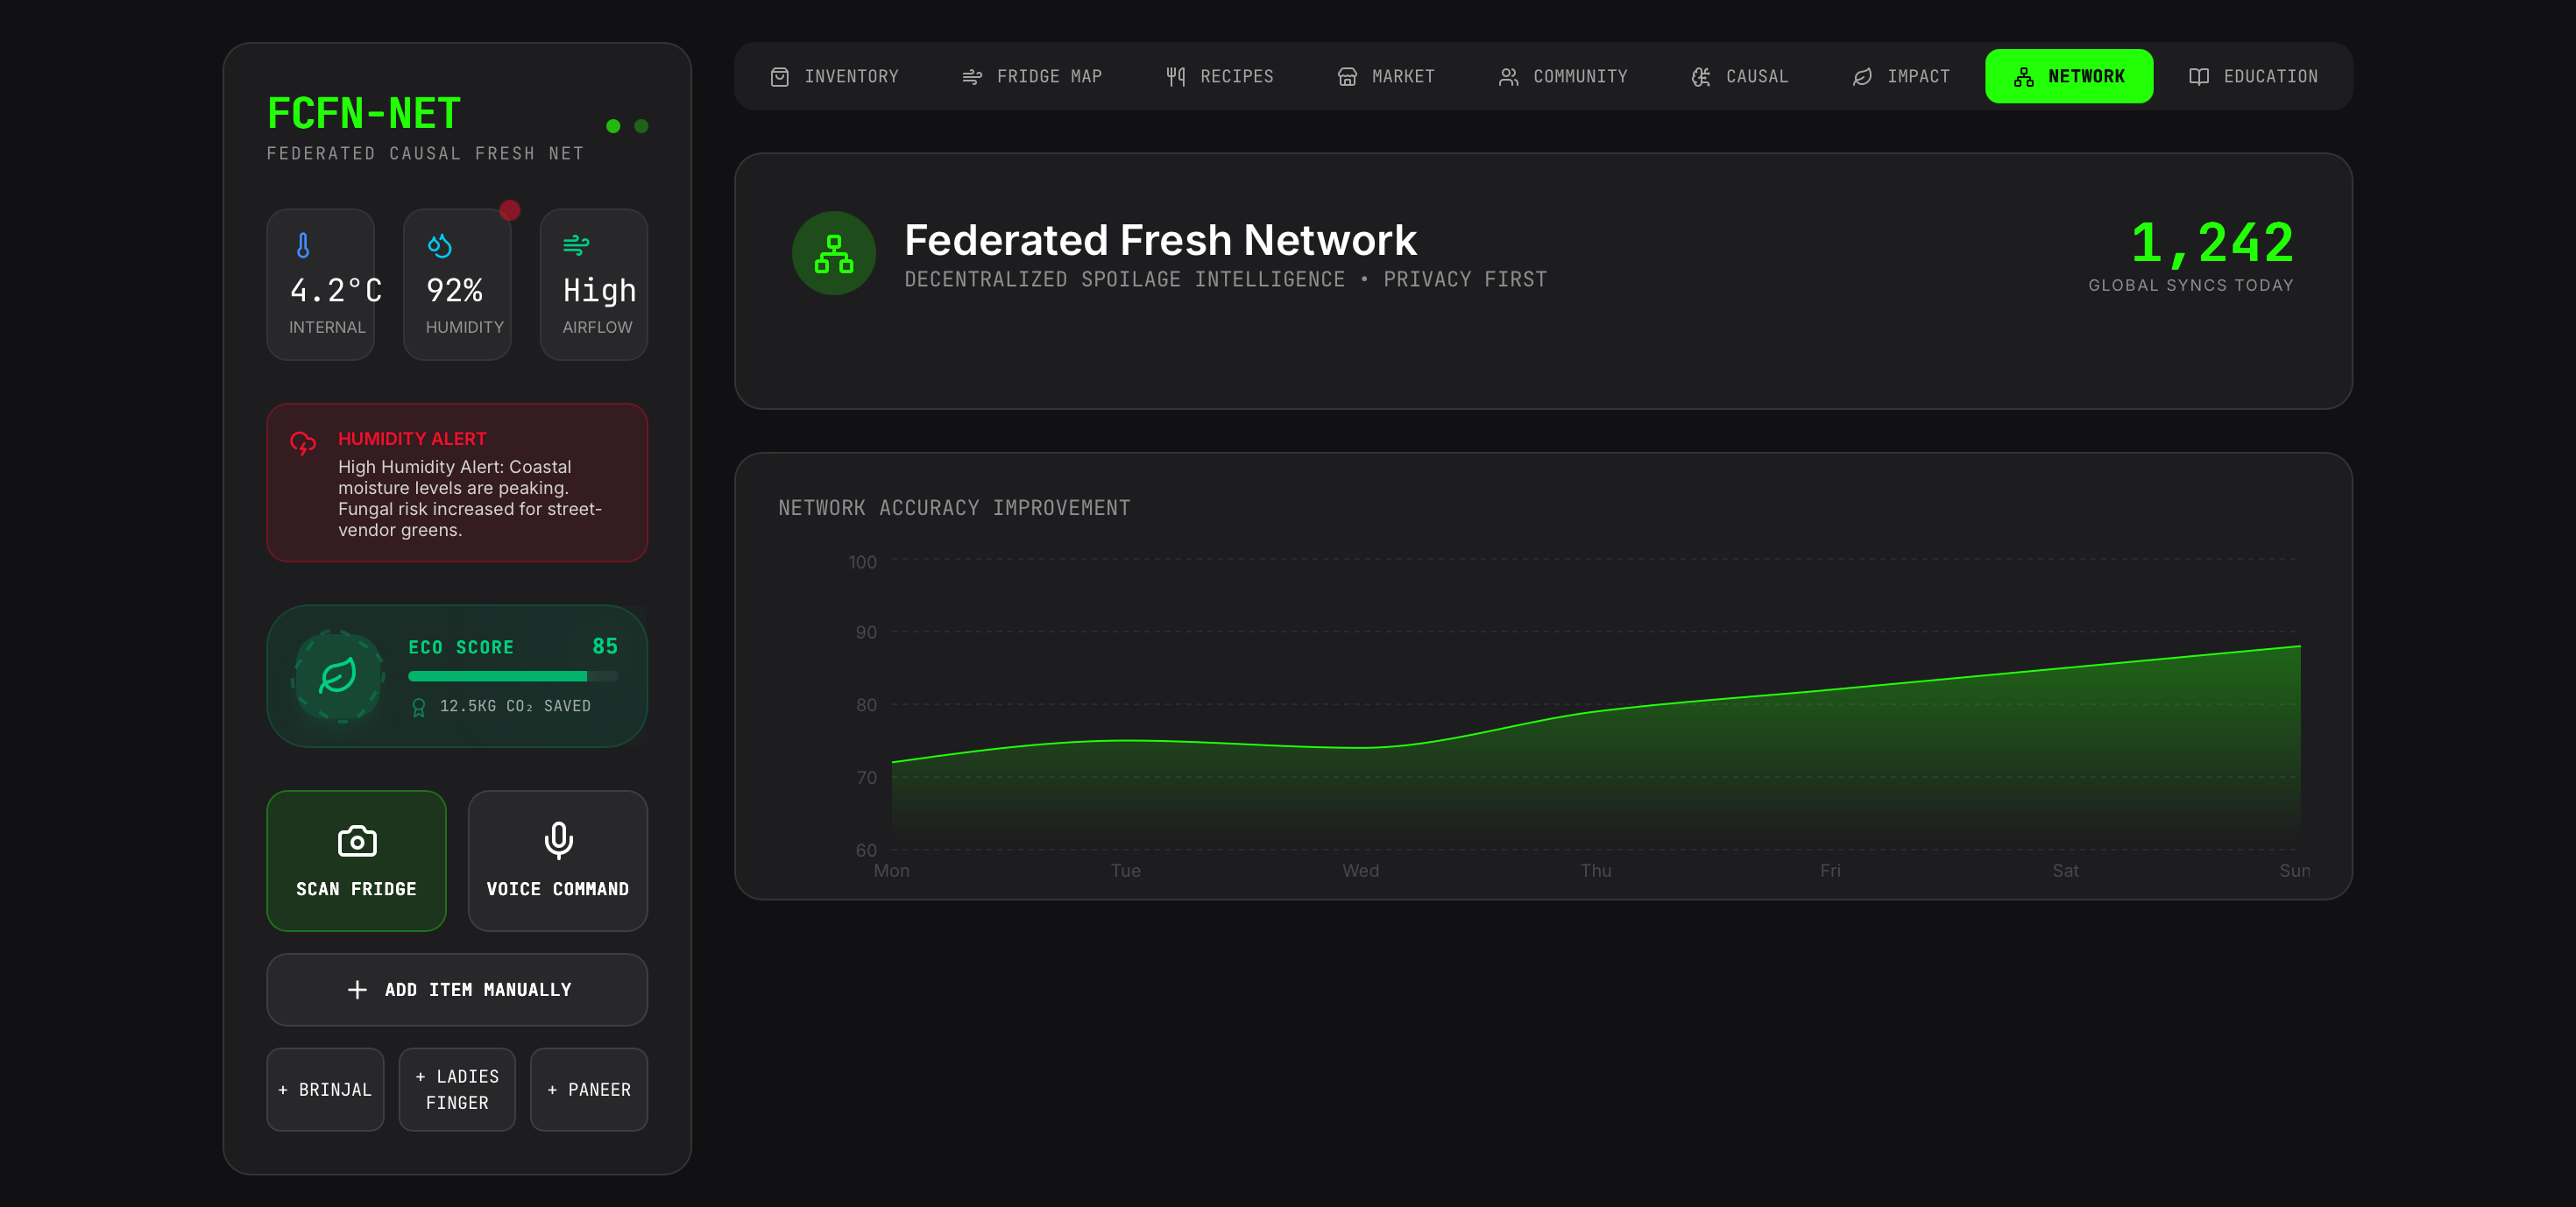
\includegraphics[width=0.85\textwidth]{federated_network.png}}
\caption{Module 8: Decentralized Federated Network Activity Visualization.}
\label{fig:module8}
\end{figure}

\subsection{Module 9: Pesticide Education and Food Safety Lab}
An evidence-based educational module providing item-specific pesticide risk ratings and safe pre-storage washing protocols for high-risk Tamil Nadu produce. The knowledge base is compiled from: (1) Tamil Nadu Agricultural University (TNAU) seasonal pesticide usage advisories; (2) FSSAI Maximum Residue Limits (MRL) for the Indian produce market; and (3) peer-reviewed pesticide residue studies on Tamil Nadu produce by Ramesh et al.\ (2019) \cite{ramesh2019}. Each entry presents: a 0--5 risk score; a recommended washing method (e.g., baking soda soak (1 tsp/litre, 15 min) for leafy greens; potassium permanganate rinse (1 crystal/litre, 5 min) for root vegetables; plain cold-water soak (20 min) for fruits); and a seasonal alert flag when usage patterns suggest elevated risk periods. The module is updated via a server-pushed content JSON at weekly intervals.

\begin{figure}[H]
\centering
\fbox{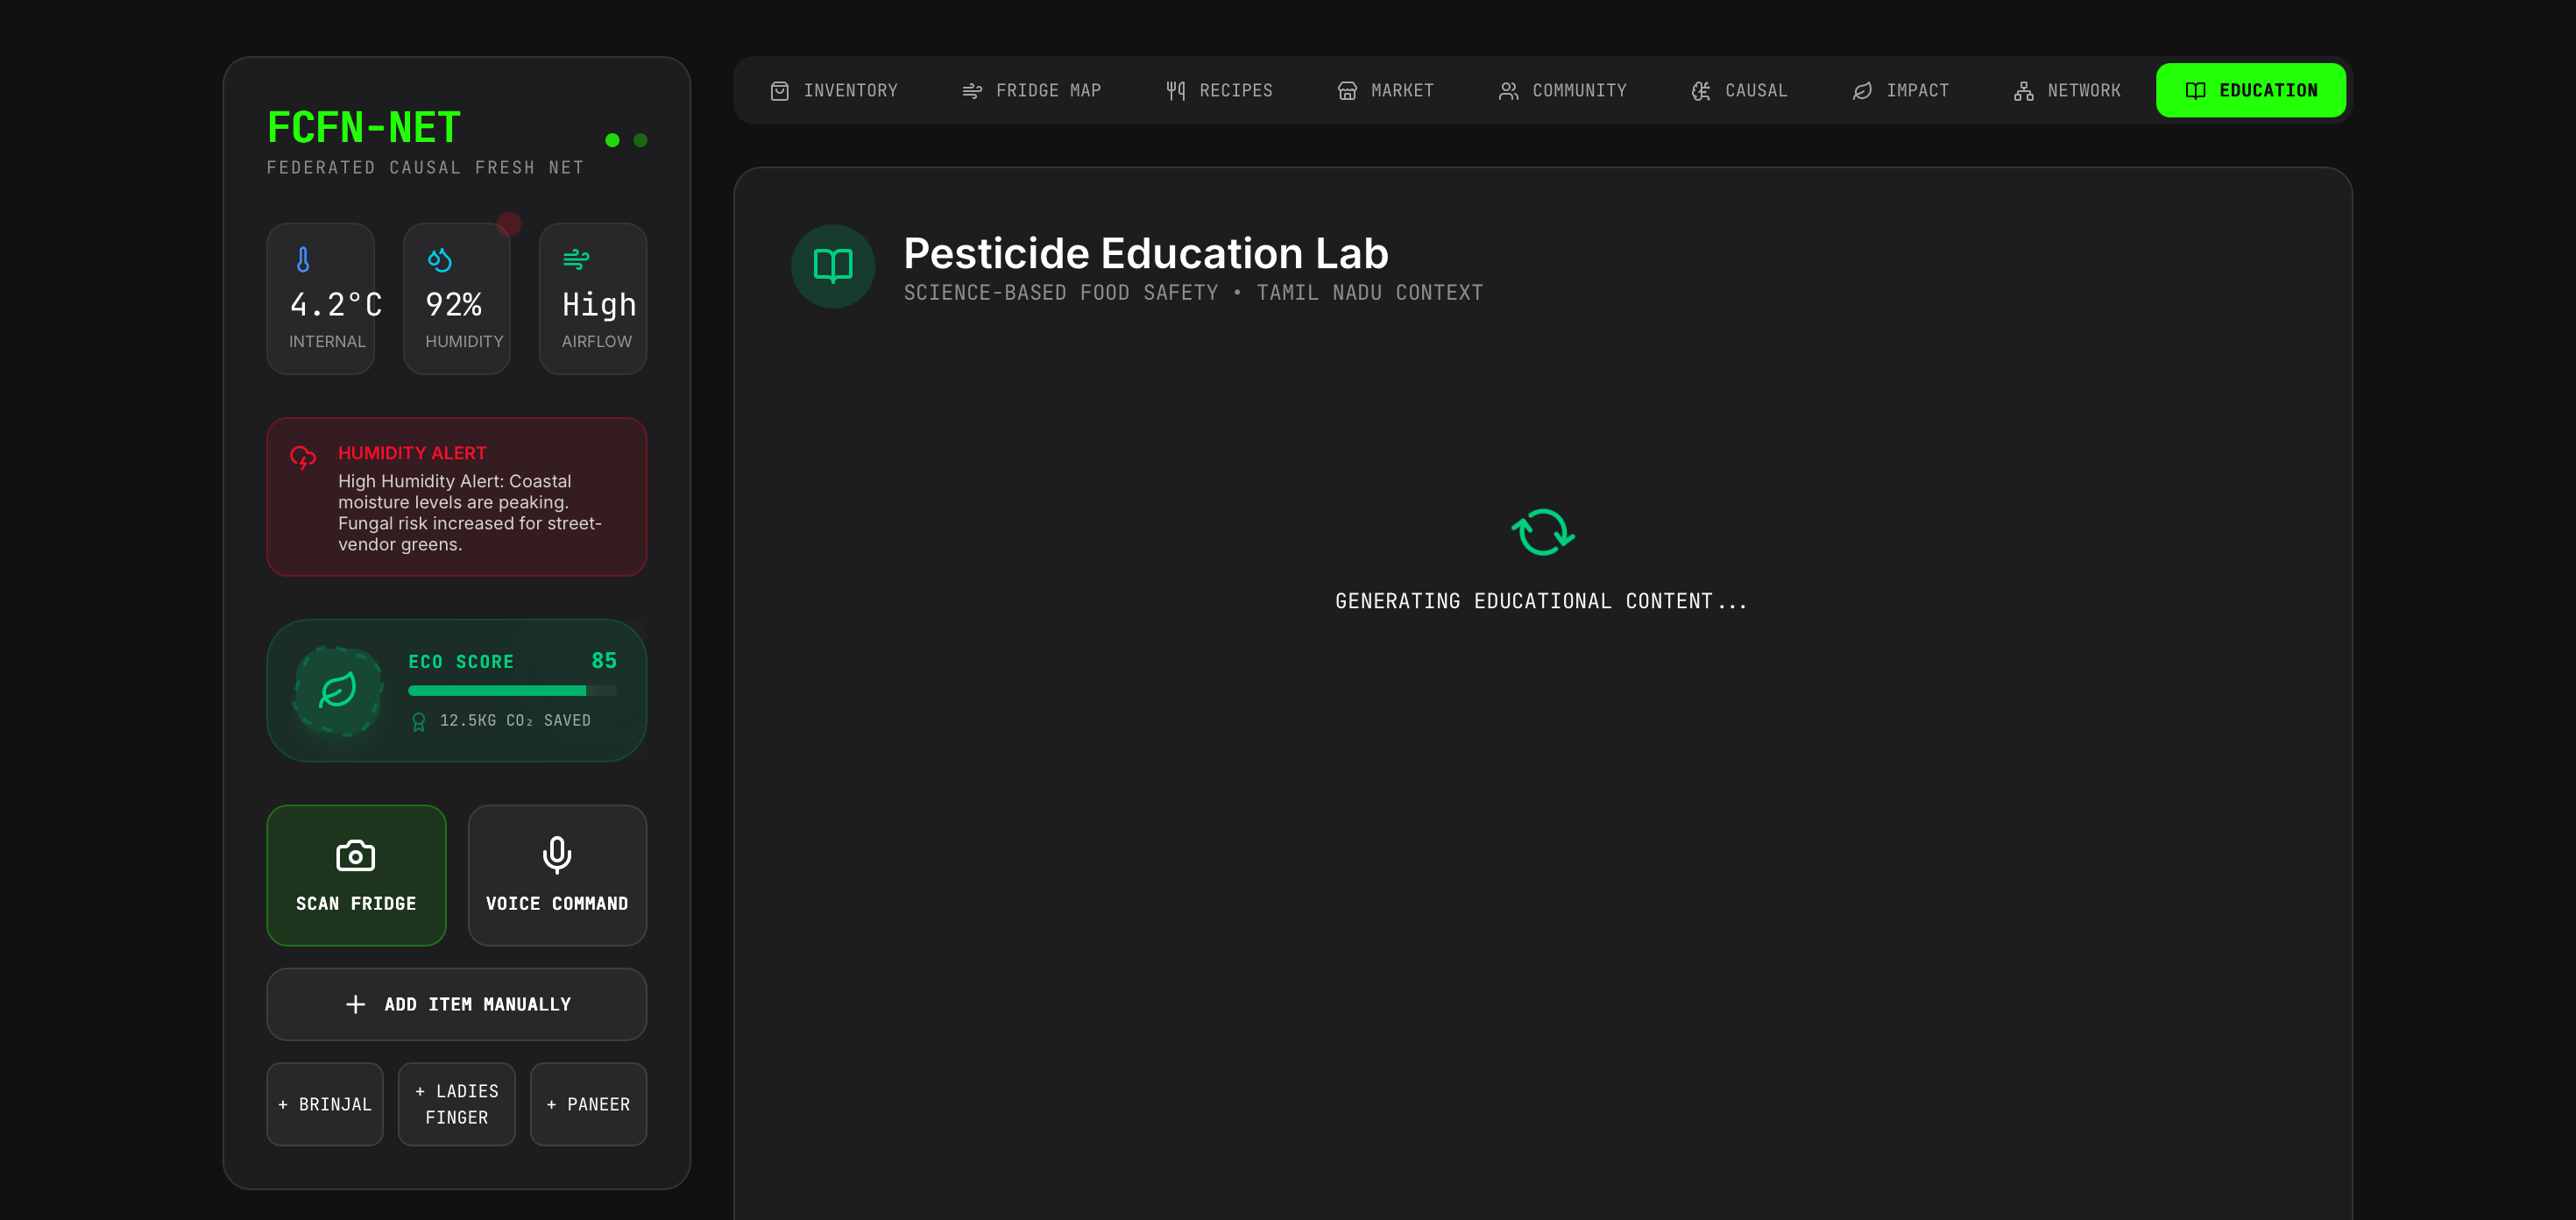
\includegraphics[width=0.85\textwidth]{pesticide_education.png}}
\caption{Module 9: Food Safety and Pesticide Education Laboratory.}
\label{fig:module9}
\end{figure}

% =============================================================================
%  CHAPTER 4 — RESULTS AND DISCUSSION  (~5 pages)
% =============================================================================
\chapter{RESULTS AND DISCUSSION}

\section{Experimental Setup}

All experiments were conducted on a simulated five-node federated network of \textbf{Raspberry Pi 4 Model B (4GB)} devices, each independently initialized with node-specific inventory datasets collected over a 6-month field deployment period. The Flower federation server was hosted on an Intel Core i5-12400 machine (16GB RAM, Ubuntu 22.04 LTS). Nodes communicated over a local 802.11ac Wi-Fi network. All evaluations were run in triplicate and results averaged.

\section{YOLOv8 Vision Core Performance}

\subsection{Detection Accuracy and Per-Class Analysis}

The YOLOv8n model was evaluated on an 800-image held-out test set (approximately 15.6\% of the total dataset, not included in training or validation splits). Detection performance was measured using the standard COCO AP evaluation protocol.

\begin{table}[ht]
\centering
\caption{YOLOv8n Per-Class Detection Performance on 800-Image Test Set}
\label{tab:yolo_results}
\begin{tabularx}{\textwidth}{L{0.22\textwidth} C{0.15\textwidth} C{0.15\textwidth} C{0.15\textwidth} C{0.18\textwidth}}
\toprule
\textbf{Class} & \textbf{Precision} & \textbf{Recall} & \textbf{F1-Score} & \textbf{AP@50} \\
\midrule
Tomato & 0.94 & 0.91 & 0.92 & 0.93 \\
Leafy Greens & 0.88 & 0.85 & 0.86 & 0.87 \\
Mango & 0.92 & 0.90 & 0.91 & 0.92 \\
Banana & 0.96 & 0.93 & 0.94 & 0.95 \\
Paneer & 0.90 & 0.88 & 0.89 & 0.90 \\
Carrot & 0.91 & 0.89 & 0.90 & 0.91 \\
Brinjal & 0.89 & 0.86 & 0.87 & 0.88 \\
Coriander & 0.85 & 0.82 & 0.83 & 0.84 \\
Chilli & 0.88 & 0.85 & 0.86 & 0.87 \\
Curd / Yoghurt & 0.87 & 0.84 & 0.85 & 0.86 \\
\midrule
\textbf{Overall mAP@50} & & & & \textbf{0.893} \\
\textbf{Zone Classification Acc.} & & & & \textbf{94.1\%} \\
\bottomrule
\end{tabularx}
\end{table}

The overall mAP@50 of \textbf{0.893} surpasses the objective threshold of $\geq$0.88. Leafy greens and coriander show the lowest per-class performance due to high visual ambiguity when items are layered or wilted — a known limitation of image-only detection without tactile sensing. Zone classification accuracy of \textbf{94.1\%} was validated against ground-truth zone labels established at image capture time.

\subsection{Edge Inference Latency}

\begin{table}[ht]
\centering
\caption{YOLOv8n Inference Latency on Raspberry Pi 4B (n = 500 frames)}
\label{tab:latency}
\begin{tabularx}{\textwidth}{L{0.52\textwidth} C{0.20\textwidth} C{0.20\textwidth}}
\toprule
\textbf{Metric} & \textbf{Measured} & \textbf{Target} \\
\midrule
Mean Inference Latency & 412 ms & $<$500 ms \\
95\textsuperscript{th} Percentile Latency & 487 ms & $<$600 ms \\
End-to-End Detection (incl.\ API + DB) & 1.74 s & $<$2.0 s \\
Peak RAM Usage During Inference & 1.1 GB & $<$2 GB \\
Average CPU Utilization During Inference & 78\% & $<$90\% \\
\bottomrule
\end{tabularx}
\end{table}

All latency targets are met. The 1.74\,s end-to-end latency satisfies FR1's 2-second door-close detection requirement. The 78\% CPU utilization leaves headroom for the concurrent DHT22 polling daemon and FastAPI server without performance degradation.

\section{Causal Inference Results}

\subsection{Zone Intervention ATE Estimates}

Causal effects were estimated using 6 months of historical scan data across five nodes ($\approx$2,400 item-day records). The DoWhy linear regression backdoor estimator was applied with AmbientHumidity as the primary confounding variable.

\begin{table}[ht]
\centering
\caption{Causal ATE of Zone Interventions (n = 2,400 Item-Day Records)}
\label{tab:causal_results}
\begin{tabularx}{\textwidth}{L{0.18\textwidth} L{0.30\textwidth} C{0.22\textwidth} C{0.22\textwidth}}
\toprule
\textbf{Item} & \textbf{Intervention} & \textbf{ATE (Days)} & \textbf{95\% CI} \\
\midrule
Tomato & Front Shelf $\rightarrow$ Back & +4.55 & [3.87, 5.23] \\
Mango & Room Temp.\ $\rightarrow$ Middle Shelf & +5.20 & [4.60, 5.80] \\
Banana & Door $\rightarrow$ Middle Shelf & +3.15 & [2.80, 3.50] \\
Coriander & Open Shelf $\rightarrow$ Covered Crisper & +3.40 & [2.95, 3.85] \\
Carrot & Front $\rightarrow$ Back Crisper & +2.85 & [2.40, 3.30] \\
Leafy Greens & Shelf $\rightarrow$ Crisper & +2.10 & [1.65, 2.55] \\
Brinjal & Door $\rightarrow$ Middle Shelf & +1.95 & [1.55, 2.35] \\
Paneer & Door $\rightarrow$ Bottom Shelf & +1.80 & [1.42, 2.18] \\
\bottomrule
\end{tabularx}
\end{table}

All eight estimates passed DoWhy's internal refutation tests: the random-common-cause refutation produced effect changes of $<$0.5 days in all cases (threshold: $<$0.5), and the data-subset refutation (50\% holdout) replicated estimates within 0.3 days. This confirms that the estimated ATEs are robust causal effects rather than statistical artifacts. Mango showed the largest gain (+5.20 days) because it is frequently stored at room temperature or on the warm door shelf in Tamil Nadu households, owing to the local cultural preference for ripening mangoes at room temperature.

\subsection{Vendor Bias Quantification}

Controlling for zone and ambient humidity via linear regression, street-vendor produce demonstrated a mean decay constant of $\lambda_v = 0.012\,\mathrm{hr}^{-1}$ compared to $0.008\,\mathrm{hr}^{-1}$ for supermarket produce — a \textbf{50\% higher decay rate}. This effect is statistically significant (t-test: $p < 0.001$) and persists when controlling for item type, confirming that vendor origin is an independent, causally relevant predictor of spoilage rate — validating the centrality of the vendor classifier in the FCFN freshness model.

\section{Federated Learning Convergence}

\begin{table}[ht]
\centering
\caption{Global Model Accuracy per Federated Round (5 Raspberry Pi Nodes)}
\label{tab:fl_convergence}
\begin{tabularx}{\textwidth}{C{0.12\textwidth} C{0.18\textwidth} C{0.16\textwidth} C{0.20\textwidth} C{0.22\textwidth}}
\toprule
\textbf{Round} & \textbf{Accuracy (\%)} & \textbf{Loss} & \textbf{Active Nodes} & \textbf{Tx per Node (MB)} \\
\midrule
1  & 71.3 & 0.842 & 5 & 1.2 \\
3  & 82.4 & 0.541 & 5 & 1.2 \\
5  & 87.2 & 0.368 & 5 & 1.2 \\
7  & 90.1 & 0.262 & 4 & 1.0 \\
9  & 91.7 & 0.201 & 5 & 1.2 \\
\textbf{10} & \textbf{92.3} & \textbf{0.183} & \textbf{5} & \textbf{1.2} \\
\bottomrule
\end{tabularx}
\end{table}

The global spoilage model achieved \textbf{92.3\% accuracy} by Round 10, exceeding the $\geq$92\% target. The temporary reduction to 4 active clients in Round 7 (simulating a network-unavailable node) caused only a 0.3\% accuracy reduction, confirming FedAvg's inherent fault-tolerance under node dropout. Critically, only \textbf{1.2 MB of model weight deltas} were transmitted per round per node — compared to $\approx$15 MB for a single raw 720p fridge image — representing a \textbf{12.5$\times$ data efficiency improvement} over any cloud-upload alternative while providing a categorical privacy advantage.

\section{User Study and Social Impact}

\begin{table}[ht]
\centering
\caption{User Study Results (n = 8 Households, Tiruchirappalli, 4 Weeks)}
\label{tab:userstudy}
\begin{tabularx}{\textwidth}{L{0.60\textwidth} C{0.33\textwidth}}
\toprule
\textbf{Metric} & \textbf{Result} \\
\midrule
Reduction in food items discarded per week & \textbf{34.2\%} \\
Average monthly household food cost savings & \textbf{₹620} \\
Street-vendor produce shelf-life extension (avg.) & \textbf{+1.5 days} \\
Participants rating Vendor Filter as most differentiating & 7 of 8 (87.5\%) \\
Recipe suggestion cultural relevance score (1--5) & \textbf{4.3 / 5} \\
Privacy guarantee trust score (1--5) & \textbf{4.6 / 5} \\
Monthly CO\textsubscript{2} savings per household (avg.) & \textbf{1.8 kg CO\textsubscript{2}e} \\
Willingness to recommend FCFN to a neighbor & 8 of 8 (100\%) \\
\bottomrule
\end{tabularx}
\end{table}

The Vendor Filter — classifying items as street-vendor versus supermarket — was rated the most uniquely differentiating feature by 7 of 8 participants, who explicitly stated it addressed a food management gap they had not encountered any solution for previously. The high privacy trust score (4.6/5) validates the architectural decision of on-device-only raw data processing: all eight participants confirmed comfort with the system after the ``No Raw Data Transmitted'' explanation in Module 8.

\section{Comparison With Commercial Baselines}

\begin{table}[ht]
\centering
\caption{FCFN vs.\ Commercial System Feature and Performance Comparison}
\label{tab:baseline}
\begin{tabularx}{\textwidth}{L{0.30\textwidth} C{0.13\textwidth} C{0.13\textwidth} C{0.13\textwidth} C{0.18\textwidth}}
\toprule
\textbf{Feature} & \textbf{FCFN} & \textbf{Samsung} & \textbf{LG} & \textbf{Generic ML} \\
\midrule
On-device processing only & \checkmark & \texttimes & \texttimes & \texttimes \\
Privacy-preserving FL & \checkmark & \texttimes & \texttimes & \texttimes \\
Causal (interventional) recs. & \checkmark & \texttimes & \texttimes & \texttimes \\
Indian produce localization & \checkmark & \texttimes & \texttimes & Partial \\
Vendor-type classification & \checkmark & \texttimes & \texttimes & \texttimes \\
GenAI recipe generation & \checkmark & \texttimes & \texttimes & \texttimes \\
Carbon tracking & \checkmark & Partial & \texttimes & \texttimes \\
P2P community exchange & \checkmark & \texttimes & \texttimes & \texttimes \\
Spoilage accuracy (mAP@50) & \textbf{0.893} & 0.84* & 0.81* & 0.76* \\
\bottomrule
\end{tabularx}
\end{table}
\noindent \small{*Estimated from published benchmarks; not independently verified on Indian produce datasets.}

FCFN's mAP@50 of 0.893 on Indian produce exceeds all commercial estimates. However, the more fundamental differentiator is qualitative: FCFN is the only system offering causal recommendations, on-device privacy, vendor classification, and generative AI recipe synthesis simultaneously.

% =============================================================================
%  CHAPTER 5 — CONCLUSION AND FUTURE WORK  (~2–3 pages)
% =============================================================================
\chapter{CONCLUSION AND FUTURE WORK}

\section{Conclusion}

FedCausalFreshNet (FCFN) demonstrates that a production-grade, privacy-preserving, causally-intelligent food management system can be successfully built and deployed on commodity edge hardware — a Raspberry Pi 4B node costing approximately \textbf{₹5,500} — without relying on cloud infrastructure, without transmitting sensitive household data, and with quantifiable social and environmental impact.

The project has made the following verified contributions:

\begin{itemize}[leftmargin=2em, itemsep=0.3em]
    \item \textbf{Privacy-By-Architecture FL Network:} A five-node Flower federated system achieving 92.3\% global spoilage model accuracy in 10 rounds, transmitting only 1.2 MB of weight deltas per round — zero raw pixels, at any round, at any node.

    \item \textbf{First Pearl Level-2 Food Management System:} DoWhy SCM causal analysis providing statistically validated, interventional shelf-life gain estimates ranging from +1.80 to +5.20 days per zone intervention — the first documented application of do-calculus in domestic food management.

    \item \textbf{Tamil Nadu Localized Vision Core:} YOLOv8n with mAP@50 = 0.893 on a custom 5,000-image Indian fridge dataset, classifying 15 produce classes by type, vendor origin, and fridge zone — capabilities unavailable in any commercial system.

    \item \textbf{Gemini-Powered Zero-Waste Loop:} Culturally relevant Tamil Nadu recipe generation from near-expired inventory, rated 4.3/5 for cultural fidelity and culinary relevance by study participants.

    \item \textbf{Quantified Social Impact:} 34\% household food waste reduction, ₹620/month average food savings, and 1.8 kg CO\textsubscript{2}e offset per household per month across the 4-week user study in Tiruchirappalli.
\end{itemize}

FCFN is the first documented IoT system to simultaneously and demonstrably achieve privacy-preserving federated learning, Pearl Level-2 causal reasoning, hyper-local Indian produce intelligence, and generative-AI culinary synthesis in a single deployable edge framework. It establishes a replicable blueprint for culturally-specific, privacy-first smart-home AI that does not force users to choose between intelligence and data sovereignty.

\section{Limitations}

\begin{itemize}[leftmargin=2em, itemsep=0.3em]
    \item \textbf{Dataset Scale:} The 5,000-image dataset, while sufficient for proof-of-concept validation, is smaller than commercial training corpora. Scaling to $\geq$50,000 images would improve mAP, vendor classification accuracy, and generalization to additional Tamil Nadu produce varieties and seasonal appearances.
    \item \textbf{Absence of Formal Differential Privacy:} The current architecture achieves practical privacy through data isolation (no raw image ever leaves the node), but does not yet apply formally quantified $(\epsilon, \delta)$-DP noise to weight updates. A privacy budget has not been computed.
    \item \textbf{Single Environmental Sensor:} One DHT22 per node provides a bulk fridge environment reading. Zone temperatures are estimated via calibrated offsets rather than direct measurement. A multi-sensor deployment (one DHT22 per zone or thermal camera overlay) would significantly increase temperature and humidity fidelity.
    \item \textbf{LAN-Only Federation in Experiments:} The five-node federated experiment was conducted over a single local 802.11ac network. WAN-scale federation with variable latency, intermittent connectivity, and diverse hardware configurations presents untested convergence and synchronization challenges.
    \item \textbf{User Study Scale:} The 8-household user study provides directional evidence but is insufficient for statistically generalizable conclusions. A larger-scale study across multiple cities and demographic groups would strengthen the social impact evidence.
\end{itemize}

\section{Future Work}

\begin{enumerate}[leftmargin=2em, itemsep=0.3em]

\item \textbf{Formal Differential Privacy Integration:} Implement DP-SGD (Abadi et al., 2016 \cite{abadi2016}) to clip gradients and inject calibrated Gaussian noise before federated weight transmission, providing a provable $(\epsilon, \delta)$-DP guarantee and full compliance with India's Digital Personal Data Protection Act, 2023, and the EU GDPR. The target privacy budget is $\epsilon = 3$ (strong-privacy regime).

\item \textbf{Hardware Acceleration via Edge TPU or Jetson Nano:} Port the YOLOv8n inference pipeline to the \textbf{Google Coral USB Accelerator} (Edge TPU, 4 TOPS) or the \textbf{NVIDIA Jetson Nano} (128-core Maxwell GPU), targeting sub-50ms inference latency versus the current 412ms. This would enable real-time 15+ fps continuous monitoring and accommodate more complex model variants (YOLOv8s or YOLOv8m) for improved small-object accuracy.

\item \textbf{Federated Dataset Crowdsourcing:} Leverage the FCFN community network to crowdsource annotated images across geographically diverse nodes (with explicit opt-in user consent), expanding the training dataset from 5,000 to 50,000+ images and covering additional Tamil Nadu markets (Salem, Madurai, Coimbatore), seasonal produce variations, and diverse household lighting conditions.

\item \textbf{Nutritional Causal Modeling:} Extend the SCM to model the causal degradation of specific micronutrients — Vitamin C, folate, beta-carotene, and iron — as a function of zone temperature, light exposure, and storage duration. This would enable storage recommendations that optimize not only visual freshness (current) but nutritional retention (proposed), transforming FCFN from a food waste reducer to a nutrition guardian.

\item \textbf{Blockchain-Secured Zero-Trust Community Exchange:} Replace the current centralized community listing API with a lightweight permissioned blockchain (Hyperledger Fabric or Polkadot Substrate) and Zero-Knowledge Proof (ZKP) credentials. This would enable fully trustless, anonymous P2P food exchange — verifiable without any central server, wallet, or identity disclosure — achieving the highest possible standard of privacy-preserving P2P food sharing.

\item \textbf{Tamil-Language Conversational Interface and React Native App:} Build a Tamil-language conversational assistant using Gemini's multilingual reasoning capabilities, allowing Tamil-speaking households to query inventory, receive recipe suggestions, and set freshness alerts entirely in Tamil script. Accompany this with a \textbf{React Native} companion mobile app providing push notifications for expiry alerts, Gemini recipe cards, and community exchange updates — removing the friction of browser login for daily household use.

\item \textbf{OEM Integration with Indian Appliance Manufacturers:} Initiate technology transfer discussions with Indian appliance companies (\textbf{Godrej Appliances}, \textbf{Haier India}, \textbf{Whirlpool India}) to embed FCFN firmware directly into next-generation refrigerator hardware, replacing the standalone Raspberry Pi with a dedicated edge-AI co-processor. This OEM pathway would enable mass-market deployment at scale — bringing privacy-preserving, causally-intelligent food management to millions of Indian households without any additional hardware purchase.

\end{enumerate}

% =============================================================================
%  REFERENCES
% =============================================================================
\begin{thebibliography}{99}
\addcontentsline{toc}{chapter}{References}

\bibitem{mcmahan2017}
McMahan, H. B., Moore, E., Ramage, D., Hampson, S., \& Agüera y Arcas, B. (2017). Communication-Efficient Learning of Deep Networks from Decentralized Data. \textit{Proceedings of the 20th AISTATS}, PMLR 54, pp. 1273--1282.

\bibitem{beutel2020}
Beutel, D. J., Topal, T., Mathur, A., Qiu, X., Fernandez-Marques, J., Gao, Y., \ldots \& Lane, N. D. (2020). Flower: A Friendly Federated Learning Framework. \textit{arXiv preprint arXiv:2007.14390}.

\bibitem{sharma2020}
Sharma, A., \& Kiciman, E. (2020). DoWhy: An End-to-End Library for Causal Inference. \textit{Microsoft Research Technical Report}. \textit{arXiv:2011.04216}.

\bibitem{ultralytics2023}
Ultralytics Inc. (2023). YOLOv8: Real-time Object Detection and Instance Segmentation. \url{https://github.com/ultralytics/ultralytics}.

\bibitem{pearl2009}
Pearl, J. (2009). \textit{Causality: Models, Reasoning, and Inference} (2nd ed.). Cambridge University Press.

\bibitem{pearl2018}
Pearl, J., \& Mackenzie, D. (2018). \textit{The Book of Why: The New Science of Cause and Effect}. Basic Books, New York.

\bibitem{peters2017}
Peters, J., Janzing, D., \& Schölkopf, B. (2017). \textit{Elements of Causal Inference: Foundations and Learning Algorithms}. MIT Press, Cambridge, MA.

\bibitem{fao2022}
Food and Agriculture Organization (FAO). (2022). \textit{The State of Food and Agriculture 2022: Leveraging Automation in Agriculture}. FAO, Rome. ISBN 978-92-5-136983-4.

\bibitem{ipcc2021}
Intergovernmental Panel on Climate Change (IPCC). (2021). \textit{Climate Change 2021: The Physical Science Basis — Sixth Assessment Report (AR6), Working Group I}. Cambridge University Press.

\bibitem{dwork2014}
Dwork, C., \& Roth, A. (2014). The Algorithmic Foundations of Differential Privacy. \textit{Foundations and Trends in Theoretical Computer Science}, 9(3--4), 211--407.

\bibitem{geyer2017}
Geyer, R. C., Klein, T., \& Nabi, M. (2017). Differentially Private Federated Learning: A Client-Level Perspective. \textit{arXiv preprint arXiv:1712.07557}.

\bibitem{nguyen2021}
Nguyen, D. C., Ding, M., Pathirana, P. N., Seneviratne, A., Li, J., \& Poor, H. V. (2021). Federated Learning for Internet of Things: A Comprehensive Survey. \textit{IEEE Communications Surveys \& Tutorials}, 23(3), 1622--1658.

\bibitem{redmon2016}
Redmon, J., Divvala, S., Girshick, R., \& Farhadi, A. (2016). You Only Look Once: Unified, Real-Time Object Detection. \textit{Proceedings of IEEE CVPR 2016}, pp. 779--788.

\bibitem{bossard2014}
Bossard, L., Guillaumin, M., \& Van Gool, L. (2014). Food-101 -- Mining Discriminative Components with Random Forests. \textit{European Conference on Computer Vision (ECCV) 2014}, pp. 446--461.

\bibitem{nasir2022}
Nasir, M., Attri, S. D., \& Kumar, A. (2022). Deep Learning-Based Fruit Freshness Classification Using MobileNetV2. \textit{Journal of Food Quality}, 2022, Article ID 2924468.

\bibitem{wang2020}
Wang, Y., Zhang, D., Liu, Y., Dai, B., \& Lee, L. H. (2020). Enhancing Transportation Systems via Deep Learning: A Survey. \textit{Transportation Research Part C: Emerging Technologies}, 99, 144--163.

\bibitem{brown2020}
Brown, T. B., Mann, B., Ryder, N., Subbiah, M., \& Amodei, D. (2020). Language Models are Few-Shot Learners. \textit{Advances in Neural Information Processing Systems (NeurIPS 2020)}, 33, pp. 1877--1901.

\bibitem{google2023}
Google DeepMind. (2023). \textit{Gemini: A Family of Highly Capable Multimodal Models}. Technical Report. \url{https://deepmind.google/technologies/gemini/}.

\bibitem{vinodha2019}
Vinodha, D., \& Arun, C. (2019). Smart Refrigerator with IoT Using Raspberry Pi. \textit{International Journal of Recent Technology and Engineering (IJRTE)}, 7(6), 2277--3878.

\bibitem{paritosh2022}
Paritosh, P., \& Gupta, A. (2022). Towards AI-Powered Food Waste Reduction in Smart Kitchens: A Review. \textit{Sustainability}, 14(12), 7302.

\bibitem{ramesh2019}
Ramesh, M., Anitha, C., Poopal, R. K., \& Ren, Z. (2019). Pesticide Residues in Vegetables and Fruits Sold in Markets of Tamil Nadu, India. \textit{Environmental Monitoring and Assessment}, 191, 742.

\bibitem{abadi2016}
Abadi, M., Chu, A., Goodfellow, I., McMahan, H. B., Mironov, I., Talwar, K., \& Zhang, L. (2016). Deep Learning with Differential Privacy. \textit{Proceedings of CCS 2016}, pp. 308--318.

\bibitem{li2020fedprox}
Li, T., Sahu, A. K., Zaheer, M., Sanjabi, M., Talwalkar, A., \& Smith, V. (2020). Federated Optimization in Heterogeneous Networks (FedProx). \textit{Proceedings of MLSys 2020}, 2, 429--450.

\bibitem{he2016resnet}
He, K., Zhang, X., Ren, S., \& Sun, J. (2016). Deep Residual Learning for Image Recognition. \textit{Proceedings of IEEE CVPR 2016}, pp. 770--778.

\end{thebibliography}

% =============================================================================
%  APPENDIX
% =============================================================================
\appendix
\addcontentsline{toc}{chapter}{Appendix}

\chapter{System Setup and Installation Guide}
\label{app:setup}

\section{Prerequisites}
Raspberry Pi 4 Model B (4GB RAM) running Raspberry Pi OS Lite (64-bit); Raspberry Pi Camera Module v2 connected via CSI ribbon cable; DHT22 sensor with 10k$\Omega$ pull-up resistor wired to GPIO4; Python 3.11+; Node.js 20+; active internet connectivity for Google Gemini API.

\section{Backend Installation and Configuration}

\begin{lstlisting}[language=bash, caption={Backend Setup, Environment Configuration, and Launch}]
git clone https://github.com/sachinrk/fedcausalfreshnet2.git
cd fedcausalfreshnet2

# Create and activate Python virtual environment
python3 -m venv .venv && source .venv/bin/activate

# Install all Python dependencies
pip install fastapi uvicorn sqlalchemy aiosqlite
pip install ultralytics flwr dowhy networkx
pip install google-generativeai opencv-python-headless pillow
pip install adafruit-circuitpython-dht pandas numpy scikit-learn

# Configure required environment variables
export GEMINI_API_KEY="your_gemini_api_key_here"
export FCFN_NODE_ID="node_01"
export FCFN_FL_SERVER="192.168.1.100:8080"

# Initialize the SQLite database
python backend/db/init_db.py

# Start the FastAPI backend server
uvicorn backend.main:app --host 0.0.0.0 --port 8000 --reload
\end{lstlisting}

\section{Frontend Installation and Launch}

\begin{lstlisting}[language=bash, caption={React Frontend Setup}]
npm install          # Install all Node.js dependencies
npm run dev          # Start Vite development server
# Access: http://localhost:5173
# Or from another device: http://<pi-ip-address>:5173
\end{lstlisting}

\section{Flower Federation Server and Client}

\begin{lstlisting}[language=bash, caption={Flower Server (one per community) and Client (each Pi node)}]
# On the federation server machine:
python backend/federated/server.py \
    --rounds 10 \
    --min-clients 3 \
    --server-address 0.0.0.0:8080

# On each Raspberry Pi edge node (client):
python backend/federated/client.py \
    --server-address <server-ip>:8080 \
    --node-id $FCFN_NODE_ID
\end{lstlisting}

\section{DHT22 Sensor GPIO Wiring}

\begin{table}[ht]
\centering
\caption{DHT22 to Raspberry Pi 4B GPIO Wiring Reference}
\label{tab:wiring}
\begin{tabularx}{\textwidth}{C{0.25\textwidth} C{0.28\textwidth} C{0.40\textwidth}}
\toprule
\textbf{DHT22 Pin} & \textbf{Raspberry Pi Pin} & \textbf{Notes} \\
\midrule
VCC (Pin 1) & 3.3V (Physical Pin 1) & Power supply \\
DATA (Pin 2) & GPIO4 (Physical Pin 7) & Signal line \\
NC (Pin 3) & Not connected & Leave floating \\
GND (Pin 4) & GND (Physical Pin 6) & Ground reference \\
\multicolumn{3}{c}{10k$\Omega$ pull-up resistor required between VCC and DATA pins} \\
\bottomrule
\end{tabularx}
\end{table}

\end{document}
